\documentclass[12pt,a4paper]{report}

% === Encodage ===
\usepackage[utf8]{inputenc}
\usepackage[T1]{fontenc}

% === Police Times New Roman (approximation LaTeX) ===
\usepackage{newtxtext,newtxmath}
\usepackage{tabularx}
\usepackage{booktabs}
% === Mise en page A4 ===
\usepackage[a4paper,margin=2.5cm]{geometry}

% === Interligne 1.5 ===
\usepackage{setspace}
\onehalfspacing

% === Tableaux propres ===
\usepackage{array}
\usepackage{longtable}
\usepackage{booktabs}
\usepackage{multirow}

% === Langue ===
\usepackage[french]{babel}
\usepackage{lmodern}

% === Flottants et images ===
\usepackage{float}
\usepackage{graphicx}

% === Mathématiques et théorèmes ===
\usepackage{amsmath, amssymb, amsfonts, mathtools}
\usepackage{amsthm}

% === TikZ pour les diagrammes ===
\usepackage{tikz}
\usetikzlibrary{positioning, arrows.meta, shapes.geometric, shapes, calc, fit, backgrounds, decorations.pathreplacing}

% === Algorithmes ===
\usepackage{algorithm}
\usepackage{algpseudocode}

% === Listes et divers ===
\usepackage{enumitem}
\usepackage{xcolor}
\usepackage{hyperref}
\usepackage{fancyhdr}

% === Définitions pour les théorèmes ===
\theoremstyle{definition}
\newtheorem{definition}{Définition}[section]
\newtheorem{propriete}{Propriété}[section]
\newtheorem{proposition}{Proposition}[section]

% === Style TikZ global ===
\tikzset{
    layer/.style={
        rectangle, draw=black!70, thick,
        minimum width=9cm, minimum height=0.9cm,
        rounded corners=2pt,
        fill=blue!5
    },
    node_state/.style={
        circle, draw=black!70, thick,
        minimum size=1.4cm,
        fill=blue!10
    },
    msg/.style={
        -{Latex[length=2mm]}, thick
    },
    timeline/.style={
        thick, -{Latex[length=2mm]}
    },
    block/.style={
        rectangle, draw, rounded corners,
        minimum width=4cm, minimum height=1cm,
        align=center
    },
    decision/.style={
        diamond, draw, aspect=2,
        align=center, inner sep=2pt
    }
}

\title{Parallax - rapport}
\author{ALAN TCHAPDA}
\date{April 2026}
\setcounter{tocdepth}{3}
\begin{document}
\tableofcontents



\chapter*{Résumé}
\addcontentsline{toc}{chapter}{Résumé}
Dans un contexte où les chercheurs en mathématiques, biologie et physique réalisent des simulations complexes et entraînent des modèles d’intelligence artificielle, les besoins en puissance de calcul sont devenus considérables. À l’ENSPY, ces travaux reposent majoritairement sur des infrastructures en ligne, coûteuses et dépendantes d’une connexion Internet souvent instable, ce qui engendre des retards significatifs. Paradoxalement, de nombreuses machines disponibles sur le campus restent sous-utilisées. Face à cette situation, le projet PARALLAX a pour objectif de fédérer ces ressources existantes afin de mettre en place une infrastructure de calcul distribué assimilable à un super-calculateur local, permettant ainsi de réduire les coûts et d’améliorer les performances d’exécution. Dans cette optique, nous avons procédé à l’identification et au diagnostic des machines disponibles, à leur remise en état lorsque nécessaire, puis à leur interconnexion au sein d’un réseau local dont la connectivité a été validée.

\textbf{Mots-clés :} calcul distribué, super-calculateur,PARALLAX.

\chapter*{Abstract}
\addcontentsline{toc}{chapter}{Abstract}

In a context where researchers in mathematics, biology, and physics carry out complex simulations and train artificial intelligence models, the demand for computing power has become substantial. At ENSPY, these tasks rely mostly on online infrastructures, which are costly and dependent on an often unstable internet connection, leading to significant delays. Paradoxically, many machines available on campus remain underutilized.

Faced with this situation, the PARALLAX project aims to federate these existing resources in order to build a distributed computing infrastructure comparable to a local supercomputer, thereby reducing costs and improving execution performance.

In this context, we carried out the identification and assessment of the available machines, restored them when necessary, and then interconnected them within a local network whose connectivity has been validated.

\textbf{Keywords:} Distributed Computing, Super-Calculator, PARALLAX.

\chapter*{Sigles et Abréviations}
\addcontentsline{toc}{chapter}{Sigles et Abréviations}

\begin{table}[H]
\centering
\begin{tabular}{ll}
\toprule
\textbf{Sigle} & \textbf{Signification} \\
\midrule

API & Application Programming Interface \\
AST & Abstract Syntax Tree \\

CLI & Command Line Interface \\
CPU & Central Processing Unit \\
DAG & Directed Acyclic Graph \\
DDR & Double Data Rate \\
DHCP & Dynamic Host Configuration Protocol \\
ENSPY & École Nationale Supérieure Polytechnique de Yaoundé \\
FIFO & First In, First Out \\
GB & Gigabyte \\
GHz & Gigahertz \\

IP & Internet Protocol \\
LAN & Local Area Network \\
LLM & Large Language Model \\
MAC & Media Access Control \\
MB & Megabyte \\
MPI & Message Passing Interface \\
RAM & Random Access Memory \\
RJ45 & Registered Jack 45 \\
SMA & Système Multi-Agent \\
TCP & Transmission Control Protocol \\
UDP & User Datagram Protocol \\
UUID & Universally Unique Identifier \\
\bottomrule
\end{tabular}
\end{table}

\chapter*{Glossaire}
\addcontentsline{toc}{chapter}{Glossaire}

\begin{itemize}

    \item[*] \textbf{Annotation} : Directive spéciale insérée dans le code source par le développeur pour indiquer au système comment décomposer et distribuer une tâche (ex : \texttt{@parallax.split}).

    \item[*]  \textbf{Contrôleur} : Nœud du cluster chargé de la supervision globale. Il reçoit les messages de heartbeat, vérifie l’état des machines en temps réel et détecte les pannes.

    \item[*] \textbf{Futex} : Mécanisme de synchronisation bas niveau permettant de bloquer un thread jusqu'à ce qu'une condition soit satisfaite, utilisé pour optimiser l’attente et la signalisation dans les systèmes concurrents.

   \item[*]  \textbf{Gossip} : Méthode de communication où chaque nœud partage régulièrement ses informations avec quelques autres nœuds choisis au hasard, ce qui permet de diffuser rapidement les informations dans tout le cluster.

    \item[*]  \textbf{Heartbeat} : Signal périodique émis par chaque nœud vers le contrôleur pour indiquer sa présence, son état et ses métriques de charge. Il permet la détection de panne et la supervision du cluster.

    \item[*]  \textbf{Horloge logique de Lamport} : Méthode simple qui permet de mettre les événements dans un ordre cohérent dans un système distribué, même si les machines n’ont pas la même heure.

    \item [*] \textbf{Nœud} : Machine physique ou virtuelle appartenant au cluster PARALLAX. Chaque nœud exécute un agent autonome capable de communiquer, de traiter des tâches et de participer aux mécanismes distribués.

    \item[*]  \textbf{Nœud maître (Master)} : Nœud du cluster chargé de la coordination globale. Il reçoit les programmes soumis, décompose les tâches, les distribue aux autres nœuds et agrège les résultats partiels.

    \item[*]  \textbf{Nœud remplaçant} : Nœud de secours destiné à reprendre immédiatement le rôle du maître ou du contrôleur en cas de panne. Il possède une capacité intermédiaire et garantit la continuité du service.

    \item[*]  \textbf{Nœud worker} : Nœud du cluster chargé d’exécuter les sous-tâches qui lui sont assignées par le maître et de renvoyer les résultats partiels.

    \item[*]  \textbf{Quorum} : Nombre minimum de nœuds nécessaires pour valider une opération distribuée, notamment une élection, généralement défini comme $\lceil N/2 \rceil + 1$.

    \item [*] \textbf{SMA (Système Multi-Agent)} : Paradigme de modélisation dans lequel chaque entité (agent) est autonome, perçoit son environnement et prend des décisions localement. Dans PARALLAX, chaque nœud agit comme un agent.

    \item[*]  \textbf{Split-brain} : Situation dans laquelle une partition du réseau conduit à l’existence simultanée de plusieurs leaders (maîtres), entraînant des incohérences dans le système.

\end{itemize}

\addcontentsline{toc}{chapter}{Liste des Figures}
\listoffigures

\addcontentsline{toc}{chapter}{Liste des Tableaux}

\listoftables

\chapter*{Introduction Générale}

Les chercheurs dans des domaines tels que les mathématiques, la biologie et la physique réalisent aujourd’hui des entraînements de modèles d’intelligence artificielle ainsi que des simulations complexes dans leurs disciplines respectives. Ces activités nécessitent une puissance de calcul très importante, généralement fournie par des infrastructures distantes telles que des serveurs en ligne ou des plateformes de calcul spécialisées.

En particulier, les chercheurs de l’ENSPY utilisent ces services en ligne, qui sont non seulement coûteux, mais également fortement dépendants de la qualité de la connexion Internet. Dans notre contexte, cette connexion est souvent lente, ce qui engendre des retards significatifs dans l’exécution des travaux. Pourtant, le campus dispose de plus de 200 machines fonctionnelles qui restent sous-exploitées.

Dès lors, une question se pose : comment fédérer les ressources matérielles existantes afin de mettre en place une infrastructure capable de réduire les coûts et de limiter les délais causés par les contraintes de connectivité, tout en offrant une solution structurée et réutilisable à travers une documentation claire destinée aux utilisateurs et aux développeurs ?

Hypothèse : la mise en place d’un supercalculateur pourrait constituer une solution à ce problème. Cependant, la réalisation d’un tel système soulève plusieurs interrogations quant à sa conception, son déploiement et surtout son utilisation, qui devra être guidée par une documentation technique permettant aux utilisateurs de programmer correctement leurs calculs sur l’infrastructure.

Le projet PARALLAX a pour objectifs :
d’exploiter les machines existantes afin de construire un supercalculateur ;
de permettre aux chercheurs d’exécuter leurs calculs sur cette infrastructure ;
et de fournir une documentation complète décrivant les interfaces, les annotations et les mécanismes nécessaires pour programmer et soumettre efficacement des tâches sur le système.

Notre méthodologie se décline en deux axes : physique et logique. Sur le plan physique, il s’agit de récupérer les machines, de diagnostiquer leurs caractéristiques, de les réparer si nécessaire, puis de les interconnecter en réseau et de tester leur connectivité. Sur le plan logique, il s’agit de développer les programmes nécessaires, de définir une architecture logicielle cohérente et de mettre en place une documentation permettant aux utilisateurs de comprendre comment coder et exécuter leurs applications sur l’infrastructure.

Dans les chapitres suivants, nous présenterons d’abord les concepts nécessaires ainsi que l’état de l’art dans le chapitre 1. Le chapitre 2 sera consacré à l’analyse et à la conception du projet. Enfin, le chapitre 3 abordera l’implémentation, les tests ainsi que la documentation technique destinée à l’utilisation du système.


\chapter{ Généralités et État de l’art}

\section{Généralités}

Cette section présente les notions fondamentales nécessaires à la compréhension de ce travail, notamment celles liées au calcul distribué, au parallélisme et aux systèmes multi-agents. Ces concepts constituent les bases théoriques sur lesquelles repose le système développé.

\subsection{Généralités}

\begin{itemize}
    \item[$\bullet$] \textbf{Calcul distribué :} Le calcul distribué désigne une approche informatique consistant à répartir l’exécution d’un calcul sur plusieurs machines interconnectées. L’objectif principal est d’améliorer les performances, la scalabilité et la tolérance aux pannes en exploitant la puissance de calcul collective d’un ensemble de nœuds \cite{tanenbaum_ds}.

    \item[$\bullet$] \textbf{Parallélisme :} Le parallélisme consiste à exécuter simultanément plusieurs opérations ou tâches afin de réduire le temps global d’exécution. Il peut être basé sur les données ou sur les instructions, selon la structure du problème à résoudre \cite{tanenbaum_ds}.

    \item[$\bullet$] \textbf{Agent :} Un agent est une entité logicielle autonome capable de percevoir son environnement, de prendre des décisions et d’agir pour atteindre des objectifs spécifiques \cite{wooldridge}.

    \item[$\bullet$] \textbf{Système multi-agents :} Un système multi-agents (SMA) est un ensemble d’agents interagissant entre eux dans un environnement partagé. Ces interactions permettent la coordination, la coopération et parfois la compétition afin de résoudre un problème global \cite{wooldridge}.

    \item[$\bullet$] \textbf{Orchestrateur :} L’orchestrateur est un composant chargé de la répartition et de la coordination des tâches entre les différents agents ou nœuds du système. Il optimise l’utilisation des ressources disponibles et assure une exécution efficace des calculs \cite{tanenbaum_ds, kubernetes}.

    \item[$\bullet$] \textbf{Contrôleur :} Le contrôleur est un nœud spécialisé chargé de la supervision continue du cluster. Il centralise les informations envoyées périodiquement par les autres nœuds (heartbeat), maintient une vue globale et actualisée de leur état (ressources disponibles, activité, connectivité) et analyse ces données afin de détecter rapidement toute anomalie ou défaillance \cite{tanenbaum_ds}.

Au-delà de la simple surveillance, le contrôleur joue un rôle clé dans la stabilité du système. Il déclenche les mécanismes de gestion des pannes, tels que la mise hors service d’un nœud défaillant ou l’initiation d’un processus d’élection pour remplacer un rôle critique \cite{bully}. Il garantit ainsi la cohérence, la fiabilité et la continuité du fonctionnement global du cluster.


    \item[$\bullet$] \textbf{Tâche :} Une tâche représente une unité de travail à exécuter dans le système. Dans un contexte distribué, une tâche peut être décomposée en sous-tâches afin d’être exécutée en parallèle sur plusieurs nœuds \cite{topcuoglu}.

    \item[$\bullet$] \textbf{Remplaçant :} Le remplaçant est un nœud du cluster désigné pour assurer la continuité du système en cas de défaillance d’un rôle critique, notamment le maître ou le contrôleur. Il se maintient en état de veille active, avec une connaissance à jour de l’état global du cluster, afin de pouvoir reprendre immédiatement les responsabilités du nœud défaillant sans interruption significative du service.

Au-delà de ce rôle de secours, le remplaçant participe au mécanisme global de tolérance aux pannes en garantissant qu’aucune fonction essentielle du système ne reste vacante. Lorsqu’il prend le relais, un processus d’élection est automatiquement déclenché pour désigner un nouveau remplaçant, assurant ainsi la pérennité et la résilience de l’architecture distribuée \cite{bully}.


    \item[$\bullet$] \textbf{Ordonnanceur :} L’ordonnanceur est responsable de la planification de l’exécution des tâches. Il décide de l’ordre et des ressources allouées à chaque tâche en fonction de critères tels que la charge ou la priorité \cite{topcuoglu}.

    \item[$\bullet$] \textbf{DAG (Directed Acyclic Graph) :} Un DAG est un graphe orienté sans cycle représentant les dépendances entre tâches. Il est utilisé pour modéliser l’ordre d’exécution dans les systèmes parallèles et distribués \cite{topcuoglu}.

    \item[$\bullet$] \textbf{Heartbeat :} Le heartbeat est un mécanisme de communication périodique par lequel chaque nœud du cluster transmet son état au contrôleur. À intervalles réguliers, il envoie un message contenant des informations telles que son identifiant, ses ressources disponibles (CPU, mémoire), ainsi que d’autres indicateurs de fonctionnement, permettant d’obtenir une vision actualisée de l’ensemble du système \cite{tanenbaum_ds, kubernetes}.

Au-delà de la simple signalisation de présence, le heartbeat constitue un élément essentiel de la supervision. Il permet au contrôleur de détecter rapidement les défaillances en cas d’absence de message dans un délai donné, d’évaluer la charge des machines et de maintenir la cohérence globale du cluster en facilitant les décisions d’orchestration et de réallocation des tâches.


    \item[$\bullet$] \textbf{Broadcast :} Le broadcast est un mécanisme de communication consistant à diffuser un message à l’ensemble des nœuds d’un système. Il est souvent utilisé pour la synchronisation ou la diffusion d’informations globales \cite{tanenbaum_ds}.
\end{itemize}
\section{État de l’art}

L’accès à des ressources de calcul à faible coût dans des environnements à connectivité limitée reste un défi majeur dans de nombreux contextes scientifiques et académiques. Plusieurs solutions concrètes ont été proposées pour répondre à ce problème. Ces solutions explorent différentes stratégies, notamment la mutualisation des ressources, la réduction des coûts ou encore l’adaptation aux contraintes réseau et aux environnements instables.

\subsection{SETI@home : calcul distribué volontaire à grande échelle}

SETI@home est un projet scientifique développé à l’Université de Californie à Berkeley \cite{seti}. Il vise à analyser des signaux radio provenant de l’espace en exploitant la puissance de calcul d’ordinateurs personnels répartis à travers le monde. L’objectif est de transformer une masse de machines hétérogènes en une infrastructure de calcul globale.

Chaque utilisateur installe un logiciel client qui télécharge des fragments de données, exécute les calculs localement, puis renvoie les résultats à un serveur central. Ce fonctionnement permet de découper une tâche globale en unités indépendantes exécutées en parallèle sur un très grand nombre de machines.

Cette architecture permet d’atteindre une puissance de calcul très importante sans infrastructure dédiée et sans investissement matériel centralisé. Elle réduit fortement les coûts et rend possibles des calculs scientifiques à grande échelle.

Cependant, le système repose entièrement sur une connectivité Internet stable et continue. Il nécessite une communication permanente pour distribuer les tâches et récupérer les résultats, ce qui introduit une forte dépendance au réseau.

\subsection{AWS Snowball : adaptation aux environnements à faible connectivité}

AWS Snowball est une solution proposée par Amazon Web Services\cite{snowball} pour transférer de grandes quantités de données dans des environnements où la bande passante est insuffisante ou instable. Elle répond principalement aux limitations liées au transfert de données volumineuses vers le cloud.

L’utilisateur copie les données sur un dispositif physique sécurisé et chiffré. Ce dispositif est ensuite transporté vers un centre de données où les informations sont intégrées dans l’infrastructure cloud.

Cette approche permet de contourner les limitations liées aux connexions lentes ou coûteuses. Elle est particulièrement utilisée dans les contextes de migration de données massives.

Cependant, cette solution reste centrée sur le transfert de données et non sur l’exécution de calculs interactifs. Elle ne permet pas un accès continu aux ressources de calcul.

\subsection{Amazon EC2 Spot Instances : réduction du coût du calcul}

Amazon EC2 Spot Instances est un service proposé par Amazon Web \cite{spot}Services permettant d’accéder à des ressources de calcul à prix réduit. Ces ressources correspondent à des machines virtuelles disponibles temporairement dans les centres de données.

Les utilisateurs exploitent ces instances pour exécuter des charges de travail intensives telles que des simulations ou des traitements batch. Ce modèle permet de réduire significativement les coûts d’exécution.

Cette approche exploite les capacités inutilisées des infrastructures cloud pour proposer des tarifs dynamiques plus faibles.

Cependant, ces ressources peuvent être interrompues à tout moment. Leur utilisation nécessite également une connexion continue au cloud.

\subsection{HTCondor : exploitation locale des ressources disponibles}

HTCondor est un système de calcul distribué développé à l’Université du Wisconsin--Madison\cite{htcondor}. Il permet de transformer un ensemble de machines locales en une plateforme de calcul partagée.

Dans les environnements académiques, il est utilisé pour exploiter les machines lorsqu’elles sont inactives. Les tâches sont planifiées automatiquement selon la disponibilité des ressources.

Cette solution repose sur une exploitation opportuniste des ressources locales. Elle réduit les coûts et limite la dépendance au réseau Internet.

Cependant, elle nécessite une gestion avancée des ressources et un système d’ordonnancement efficace.

\section{Bilan et positionnement}

\subsection{Bilan}

\subsubsection{Étude de l’existant}

Les solutions existantes proposent différentes approches pour réduire le coût du calcul et améliorer la gestion des contraintes réseau. Certaines reposent sur la mutualisation massive des ressources distribuées, tandis que d’autres exploitent des ressources locales ou des modèles économiques flexibles dans le cloud.

Cependant, ces solutions présentent des limites importantes dans des environnements académiques à ressources contraintes. Les approches cloud restent fortement dépendantes d’une connectivité Internet stable. Les solutions de calcul distribué à grande échelle nécessitent également une infrastructure globale et une coordination permanente. Enfin, les solutions locales sont souvent limitées à des environnements fortement structurés et difficiles à généraliser.

Afin de comparer ces approches, les critères suivants sont utilisés : réduction du coût, dépendance au réseau et exploitation des ressources locales.

\begin{table}[h]
\centering
\renewcommand{\arraystretch}{1.3}
\begin{tabular}{|l|c|c|c|c|}
\hline
\textbf{Critères} & \textbf{SETI@home} & \textbf{AWS Snowball} & \textbf{EC2 Spot} & \textbf{HTCondor} \\
\hline
Réduction du coût & \checkmark & $\times$ & \checkmark & \checkmark \\
\hline
Faible dépendance réseau & $\times$ & \checkmark & $\times$ & \checkmark \\
\hline
Exploitation locale & $\times$ & $\times$ & $\times$ & \checkmark \\
\hline
\end{tabular}
\caption{Comparaison des solutions existantes}
\end{table}

\textbf{Légende :} \checkmark\ : satisfait \quad $\times$\ : non satisfait

\subsection{Positionnement}

Ce projet se positionne comme une solution de calcul distribuée locale adaptée aux environnements académiques à ressources limitées.

Contrairement aux solutions cloud comme EC2 Spot Instances, il ne dépend pas d’une connexion Internet continue. Contrairement aux approches de calcul distribué global comme SETI@home, il n’exige pas une infrastructure mondiale ni des utilisateurs externes. Enfin, contrairement aux solutions de transfert physique comme AWS Snowball, il permet l’exécution directe des tâches de calcul.

L’approche proposée exploite des machines locales inutilisées afin de constituer un cluster de calcul distribué. Elle vise à réduire les coûts d’infrastructure tout en assurant une autonomie vis-à-vis de la connectivité Internet.

Cette solution est particulièrement adaptée aux environnements académiques où des ressources matérielles existent mais restent sous-utilisées.

\chapter{Analyse et conception}

\section{Analyse}

Face à la dépendance coûteuse des chercheurs de l'ENSPY envers des serveurs distants et aux limitations d'une connectivité Internet insuffisante, le projet PARALLAX se propose de fédérer les ressources des machines sous-utilisées du campus en une infrastructure de calcul distribué locale. Pour mener à bien cette solution, nous avons procédé à une analyse selon deux axes : d'une part l'axe matériel, qui dresse l'inventaire des machines disponibles pour constituer le cluster, et d'autre part l'axe logiciel, qui permet l'identification des acteurs du système et de leurs besoins fonctionnels.

% ============================================================
\subsection{Analyse matérielle du cluster PARALLAX}
% ============================================================

\subsubsection{Les machines DELL}

Le cluster dispose de trois ordinateurs de bureau DELL. Deux d'entre eux sont des Dell OptiPlex 380 et le troisième est un Dell System 360.

\textbf{Dell OptiPlex 380 — Machine 1}
\begin{figure}[H]
    \centering
    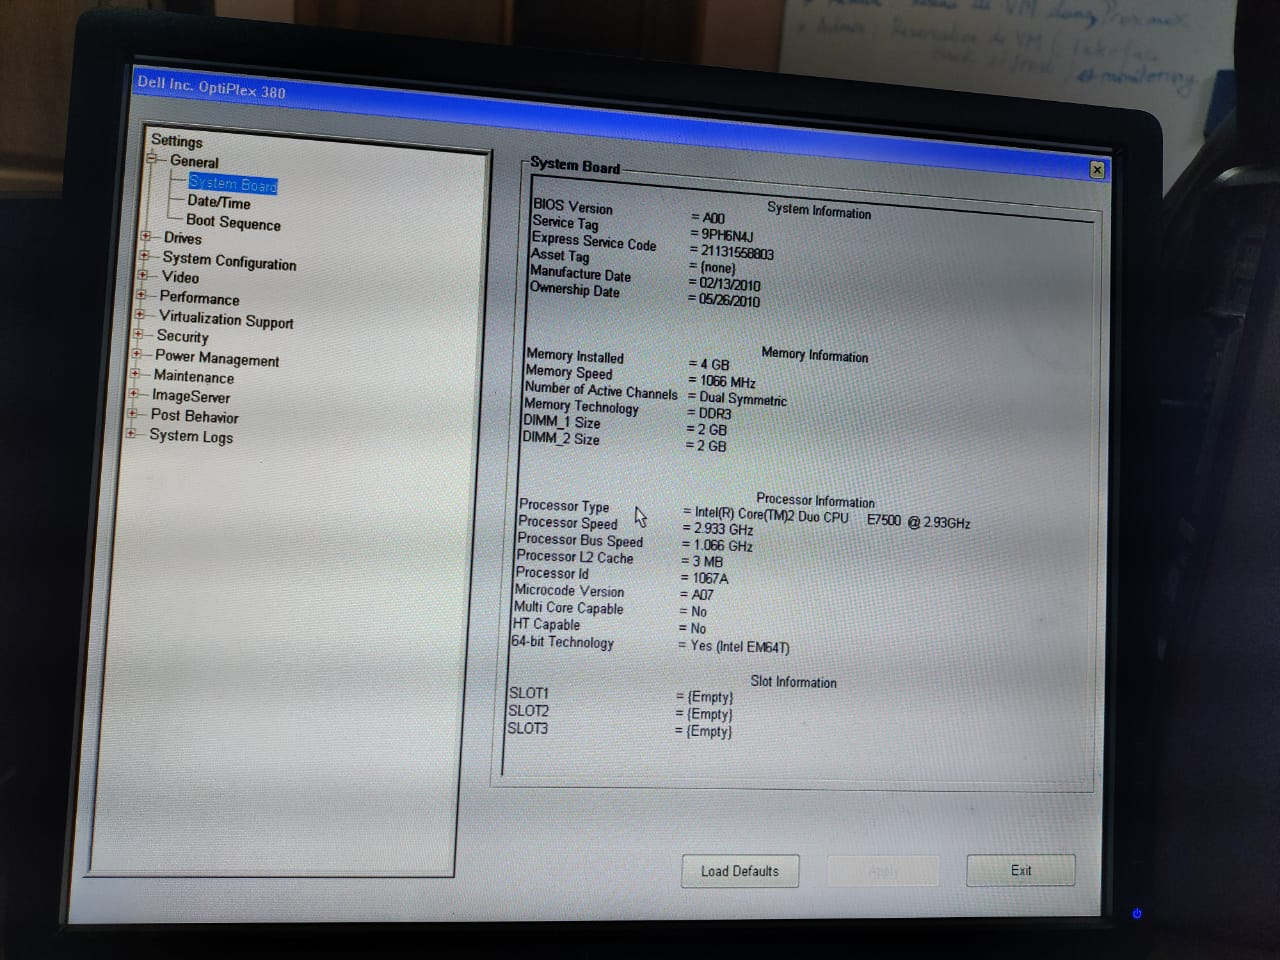
\includegraphics[width=0.5\textwidth]{images/dell_optiplex_380_m1.jpg}
    \caption{Dell OptiPlex 380 — Machine 1}
    \label{fig:dell_m1}
\end{figure}
Le processeur est un Intel Core 2 Duo E7500 cadencé à 2,933 GHz, doté de 2 cœurs physiques et d'un cache L2 de 3 MB. La mémoire RAM est de 4 GB de type DDR3 à 1066 MHz, répartie en deux barrettes de 2 GB chacune en mode Dual Symmetric. La machine supporte la technologie 64 bits.

\textbf{Dell OptiPlex 380 — Machine 2}
\begin{figure}[H]
    \centering
    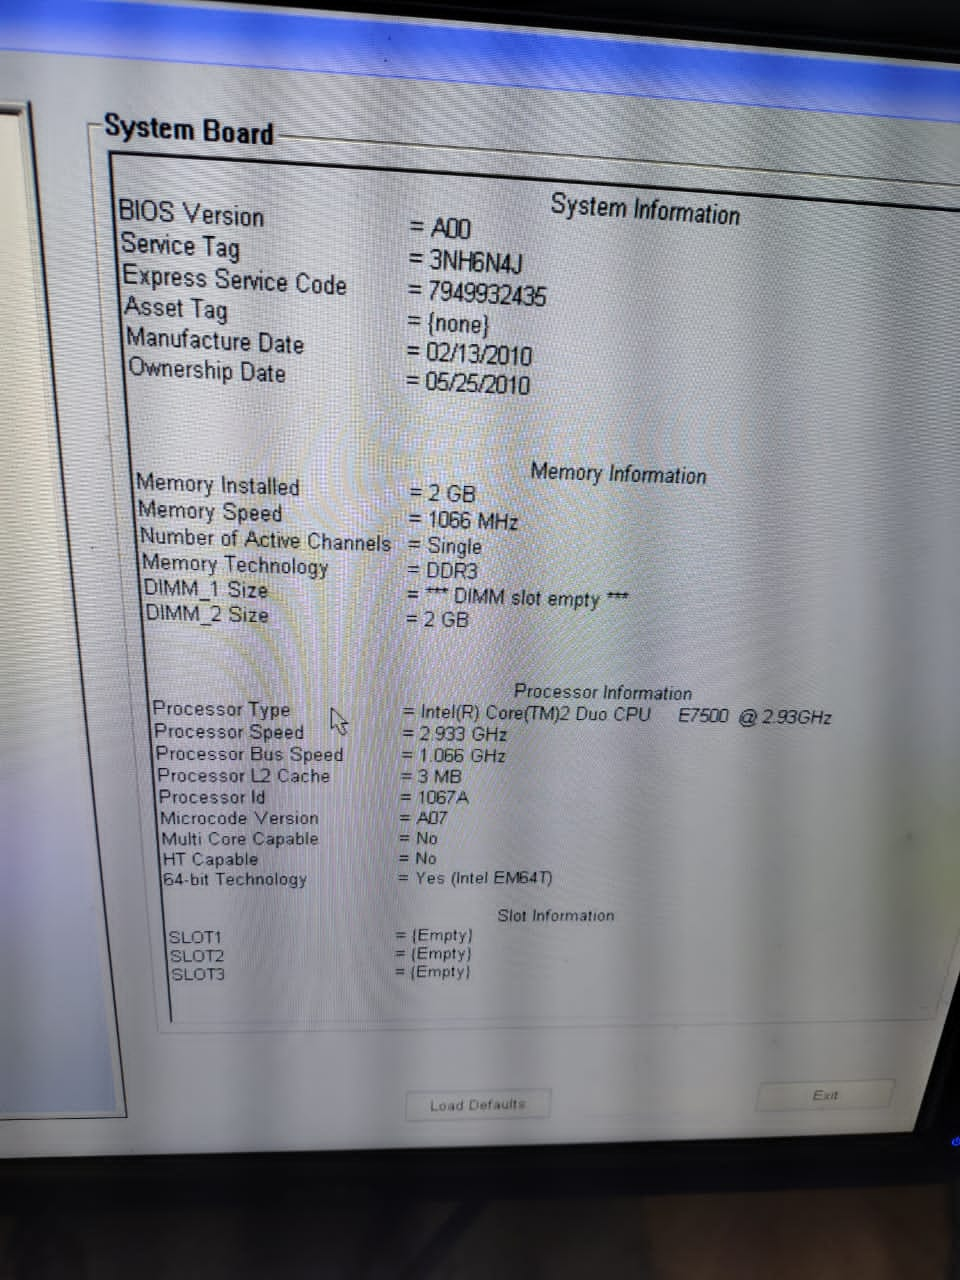
\includegraphics[width=0.5\textwidth]{images/dell_optiplex_380_m2.jpg}
    \caption{Dell OptiPlex 380 — Machine 2}
    \label{fig:dell_m2}
\end{figure}
Le processeur est identique au premier : Intel Core 2 Duo E7500 à 2,933 GHz, 2 cœurs, cache L2 de 3 MB. La mémoire RAM est de 2 GB de type DDR3 à 1066 MHz, mais un seul slot DIMM est occupé, le premier slot étant vide. La machine fonctionne en mode Single Channel, ce qui réduit les performances mémoire par rapport à la première machine.

\textbf{Dell System 360 — Machine 3}
\begin{figure}[H]
    \centering
    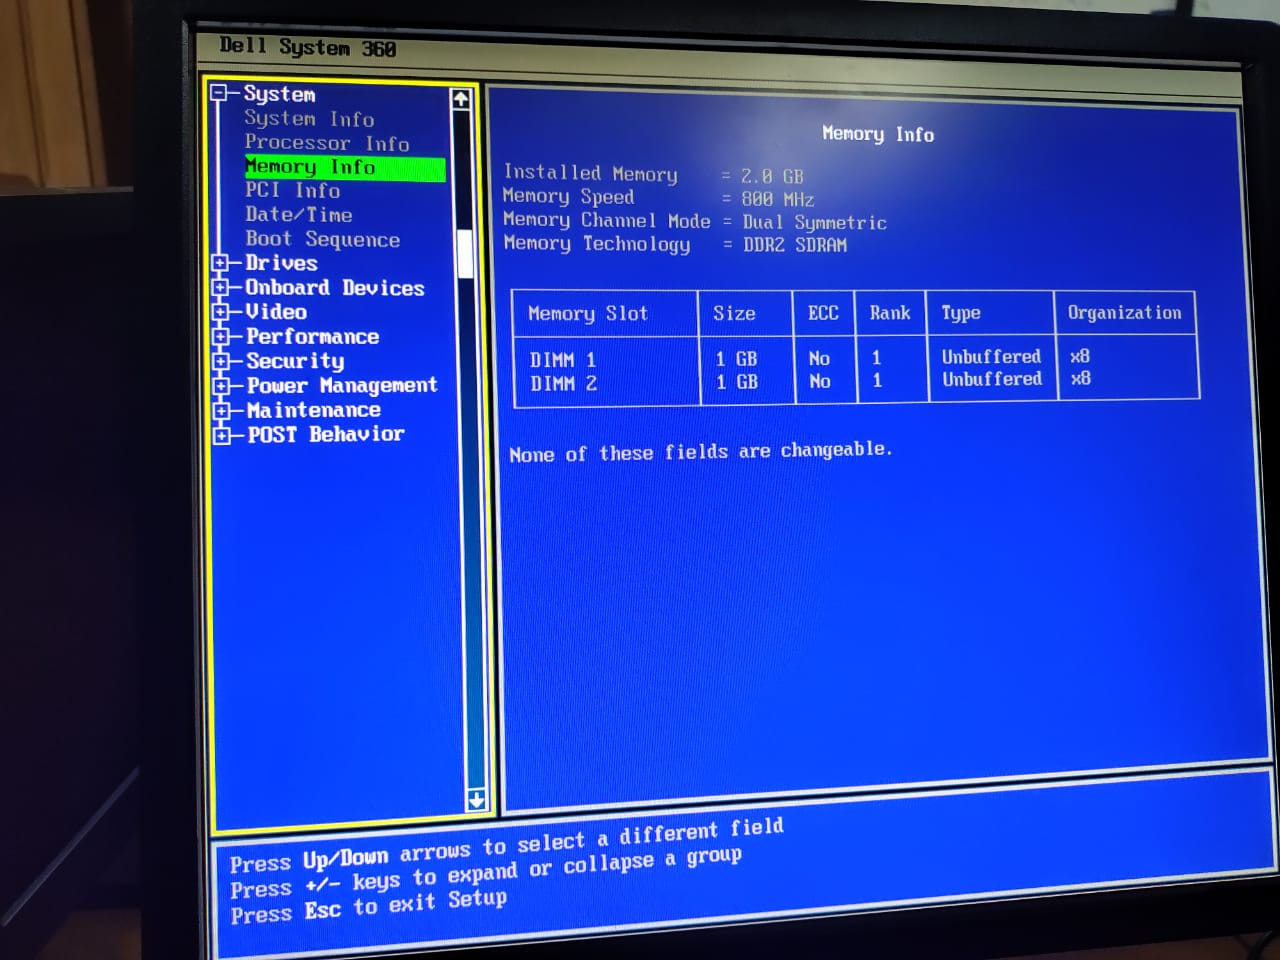
\includegraphics[width=0.5\textwidth]{images/dell_system_360_m3.jpg}
    \caption{Dell System 360 — Machine 3}
    \label{fig:dell_m3}
\end{figure}
La mémoire RAM est de 2 GB de type DDR2 à 800 MHz, répartie en deux barrettes de 1 GB chacune en mode Dual Symmetric. La technologie mémoire DDR2 est une génération en dessous des deux OptiPlex 380, ce qui implique une bande passante mémoire inférieure.

% ------------------------------------------------------------
\subsubsection{Les mini-ordinateurs}
% ------------------------------------------------------------

Le cluster intègre également trois thin clients de type Wyse. Deux d'entre eux sont équipés d'un processeur à 533 MHz, de 32 MB de RAM et de 32 MB de stockage flash. Le troisième, de gamme supérieure, dispose d'un processeur à 1 GHz, de 64 MB de RAM et de 64 MB de stockage flash. Ces trois appareils fonctionnent sous Windows CE et sont structurellement différents des postes DELL : leur faible capacité de traitement les exclut du rôle de coordinateur et les cantonne à des tâches légères de calcul au sein du cluster.

\textbf{Tiny Client ×2 (533 MHz)}
\begin{figure}[H]
    \centering
    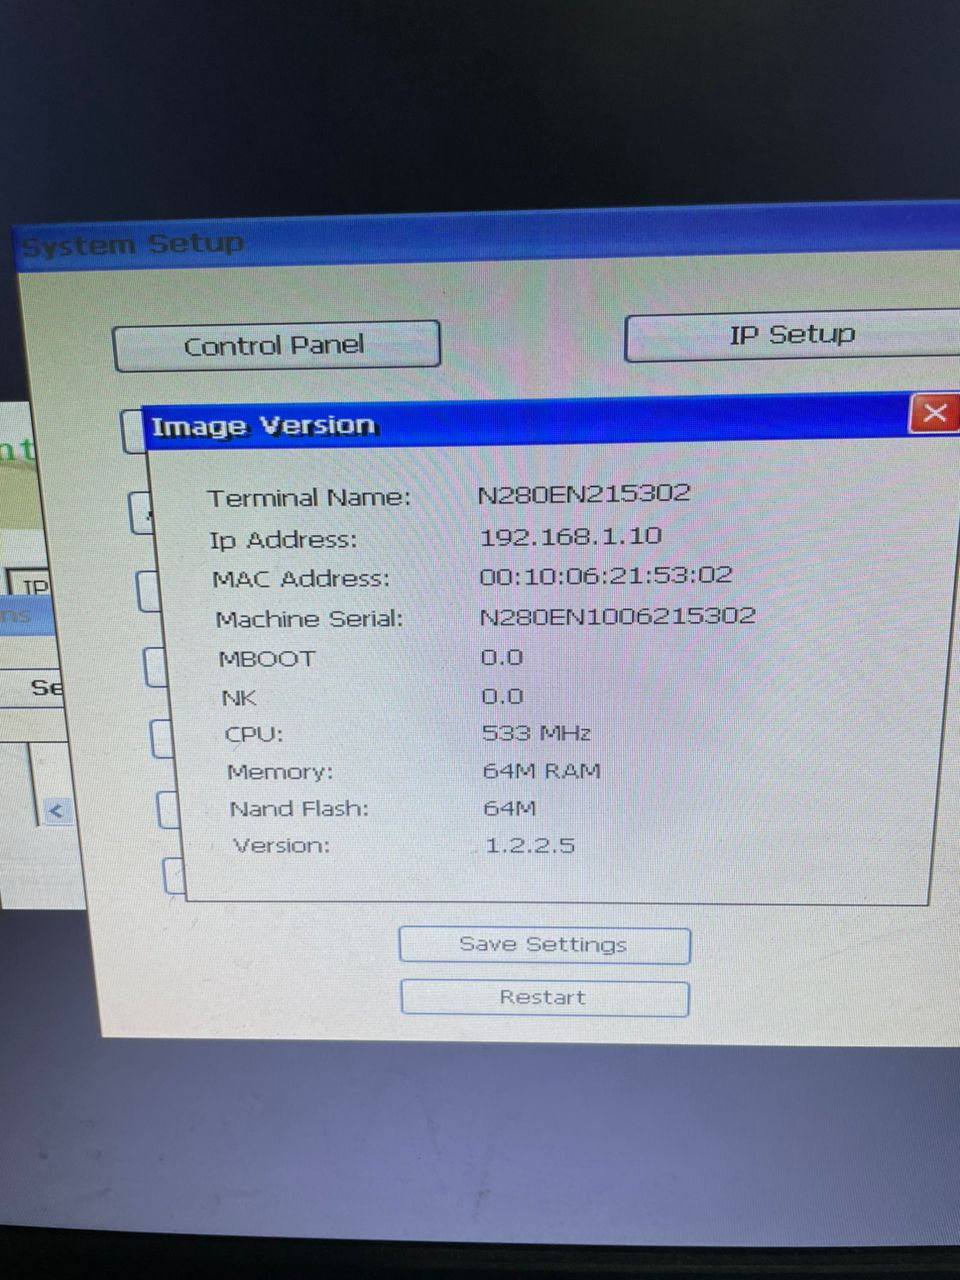
\includegraphics[width=0.5\textwidth]{images/tiny_client_533.jpg}
    \caption{Thin client Wyse — 533 MHz (×2)}
    \label{fig:tiny_533}
\end{figure}

\textbf{Tiny Client Wyse (1 GHz)}
\begin{figure}[H]
    \centering
    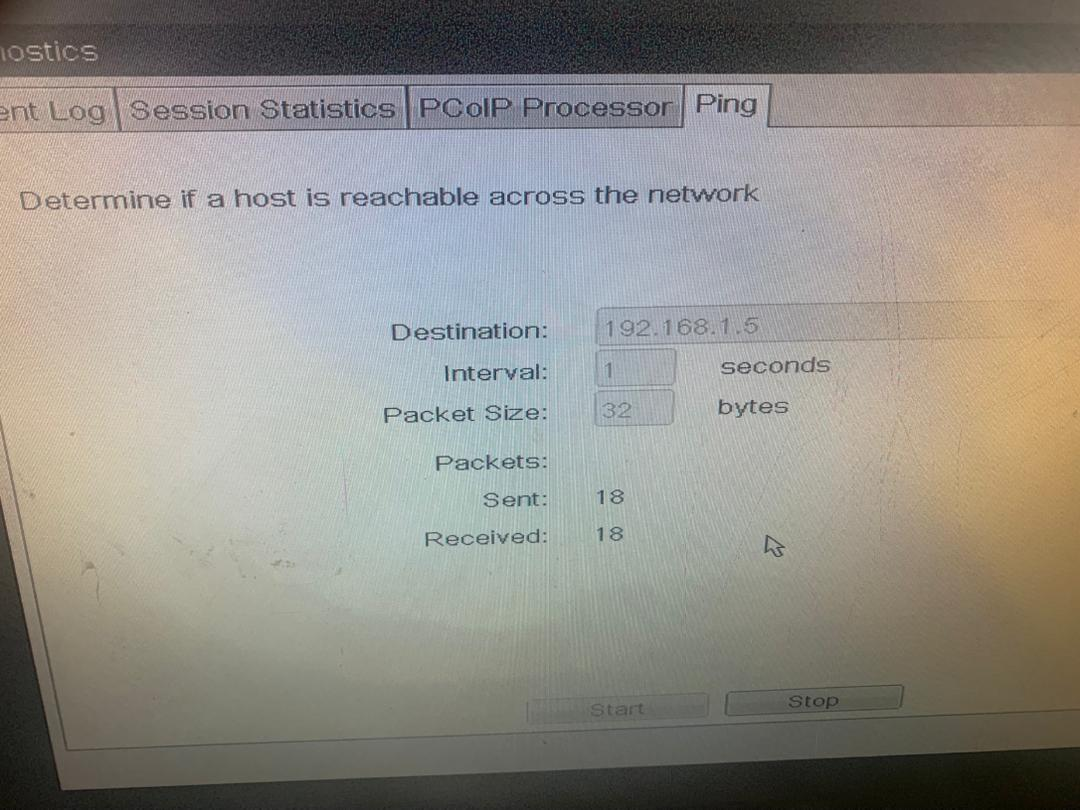
\includegraphics[width=0.5\textwidth]{images/tiny_client_wyse_1ghz.jpg}
    \caption{Thin client Wyse — 1 GHz}
    \label{fig:tiny_1ghz}
\end{figure}

% ------------------------------------------------------------
\subsubsection{Infrastructure réseau}
% ------------------------------------------------------------

Les machines sont interconnectées via un switch Ethernet à 5 ports. Six câbles réseau droits RJ45 ont été sertis manuellement par l'équipe pour les besoins du projet. Les tests de connectivité réalisés via des commandes ping entre toutes les machines ont été concluants, validant ainsi la couche physique du réseau sur laquelle repose l'ensemble de l'architecture logicielle de PARALLAX.

\begin{figure}[H]
    \centering
    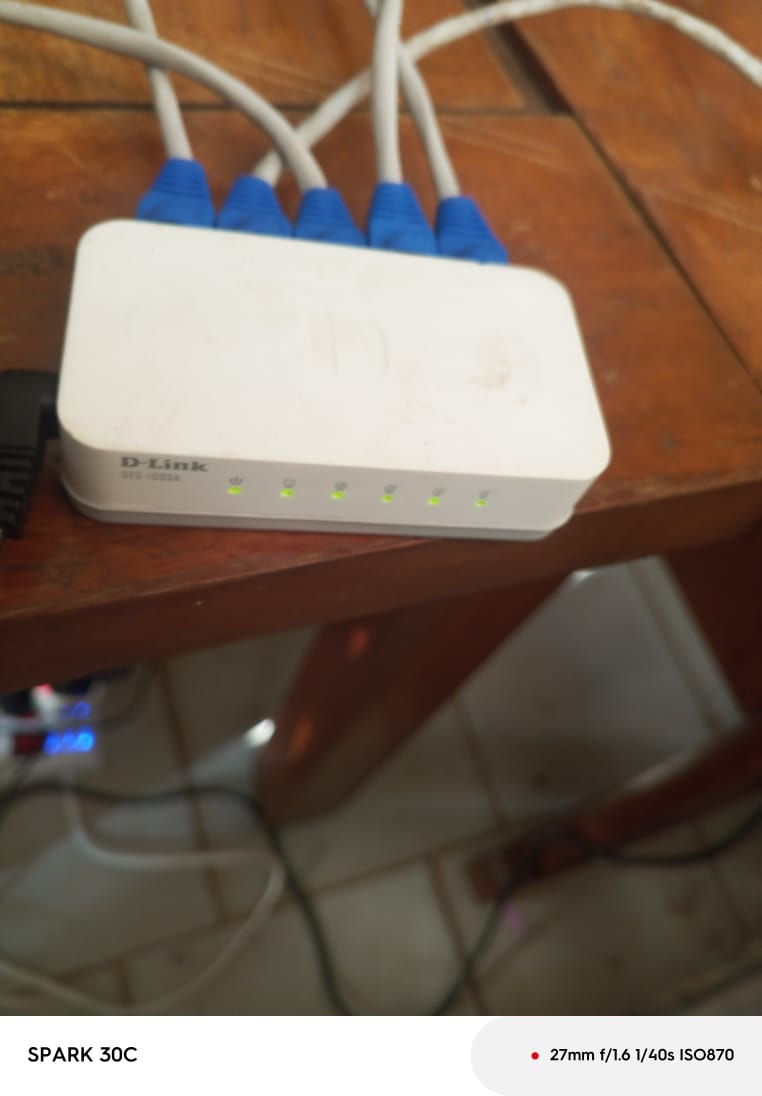
\includegraphics[width=0.5\textwidth]{switch_reseau.jpeg}
    \caption{Switch Ethernet 5 ports et câbles RJ45 sertis manuellement}
    \label{fig:switch}
\end{figure}

% ------------------------------------------------------------
\subsubsection{Récapitulatif du matériel}
% ------------------------------------------------------------

Le tableau ci-dessous résume les caractéristiques de l'ensemble des machines constituant le cluster :

\begin{table}[H]
\centering
\resizebox{\textwidth}{!}{%
\begin{tabular}{|l|l|l|l|l|l|}
\hline
\textbf{Caractéristique} & \textbf{DELL OptiPlex 380 — M1} & \textbf{DELL OptiPlex 380 — M2} & \textbf{DELL System 360 — M3} & \textbf{Tiny Client ×2} & \textbf{Tiny Client Wyse} \\
\hline
Processeur & Intel Core 2 Duo E7500 & Intel Core 2 Duo E7500 & Non visible & — & — \\
\hline
Fréquence & 2,933 GHz & 2,933 GHz & — & 533 MHz & 1 GHz \\
\hline
Nombre de cœurs & 2 & 2 & — & — & — \\
\hline
Cache L2 & 3 MB & 3 MB & — & — & — \\
\hline
RAM totale & 4 GB & 2 GB & 2 GB & 32 MB & 64 MB \\
\hline
Type de RAM & DDR3 1066 MHz & DDR3 1066 MHz & DDR2 800 MHz & — & — \\
\hline
Mode mémoire & Dual Symmetric & Single Channel & Dual Symmetric & — & — \\
\hline
Stockage & — & — & — & 32 MB flash & 64 MB flash \\
\hline
Architecture & 64 bits & 64 bits & — & — & — \\
\hline
Système d'exploitation & Ubuntu Server 18.04 & Ubuntu Server 18.04 & Ubuntu Server 18.04 & Windows CE & Windows CE \\
\hline
Rôle dans le cluster & Maître / Worker & Maître / Worker & Maître / Worker & Worker léger & Worker léger \\
\hline
\end{tabular}
}
\caption{Caractéristiques des machines du cluster PARALLAX}
\end{table}

% ------------------------------------------------------------
\subsubsection{Limites matérielles par rapport au projet}
% ------------------------------------------------------------

\textbf{Hétérogénéité des systèmes d'exploitation.} Les trois DELL fonctionnent sous Ubuntu Server 18.04 tandis que les trois thin clients fonctionnent sous Windows CE. Cette différence impose à PARALLAX de gérer une couche de sérialisation des données assurant l'interopérabilité entre les deux systèmes.

\textbf{Puissance de calcul limitée des DELL.} Les processeurs Intel Core 2 Duo datent de 2010 et ne disposent que de 2 cœurs physiques chacun. Le bénéfice du parallélisme sera donc limité par la faible puissance individuelle de chaque nœud.

\textbf{Hétérogénéité des DELL entre elles.} La première machine dispose de 4 GB de RAM en Dual Channel, la deuxième de 2 GB en Single Channel, et la troisième de 2 GB de DDR2 moins rapide. Cette hétérogénéité justifie le recours au score pondéré dans l'algorithme de vote pour l'élection du nœud remplaçant.

\textbf{Capacité très limitée des thin clients.} Avec 32 à 64 MB de RAM et des processeurs entre 533 MHz et 1 GHz, ces machines sont donc défavorisées dans le processus d'élection du remplaçant et participent au cluster uniquement pour des tâches légères.

\textbf{Contrainte du switch à 5 ports.} Cette contrainte fixe le nombre maximum de nœuds actifs dans cette première phase du projet. Toute extension nécessiterait le remplacement du switch par un modèle de plus grande capacité.

\textbf{Absence de redondance réseau.} Le switch constitue un point de défaillance unique au niveau de la couche physique. Sa défaillance entraînerait la perte totale de connectivité du cluster, indépendamment de la robustesse de la couche logicielle.

% ============================================================
\subsection{Analyse logicielle}
% ============================================================

\subsubsection{ Synthèse des intervenants et fonctionnalités}

Le système PARALLAX implique deux catégories d'acteurs.
\begin{enumerate}
    \item e \textbf{Chercheur} (étudiant, enseignant ou chercheur de l'ENSPY) soumet ses programmes annotés via une interface CLI et consulte les résultats d'exécution. 
    \item . Le \textbf{Gestionnaire de cluster} administre l'infrastructure via une interface Web : il supervise l'état des nœuds grâce aux heartbeats, et gère l'ajout ou le retrait de machines du cluster.
\end{enumerate}
\subsubsection{ Diagramme de contexte}
% ------------------------------------------------------------

\begin{figure}[H]
    \centering
    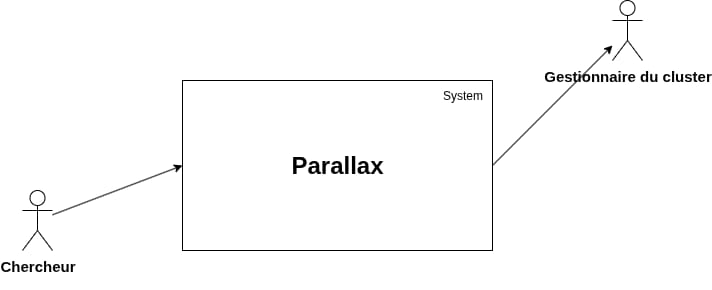
\includegraphics[width=1\textwidth]{images/parallax - diagramme de context.jpeg}
    \caption{Diagramme de Contexte}
    \label{fig:diagramme_contexte}
\end{figure}

% ------------------------------------------------------------

% ------------------------------------------------------------
\subsubsection{ Fonctionnalités et exigences}
% ------------------------------------------------------------

\subsubsection*{ Exigences fonctionnelles et non fonctionnelles}

\textbf{Exigences fonctionnelles :}
\begin{itemize}
    \item [$\bullet$]Soumission et exécution distribuée de tâches de calcul (Chercheur).
    \item [$\bullet$Import et annotation de programmes via interface CLI (Chercheur).
    \item [$\bullet$Consultation des résultats d'exécution avec détails (durée, date) (Chercheur).
    \item [$\bullet$Supervision en temps réel de l'état des nœuds via interface Web (Gestionnaire de cluster).
    \item[$\bullet$ Gestion dynamique du cluster : ajout et retrait de machines (Gestionnaire de cluster).
\end{itemize}

\textbf{Exigences non fonctionnelles :}
\begin{itemize}
    \item[$\bullet$ Résilience aux pannes : détection automatique et réaffectation des tâches, y compris en cas de surcharge d'un nœud.
    \item[$\bullet$ Transparence pour le développeur : parallélisation via annotations sans gestion manuelle du réseau.
    \item [$\bullet$Légèreté : adaptation aux petits clusters hétérogènes à ressources modestes.
    \item[$\bullet$ Performance : optimisation de la distribution des tâches en fonction d’un score pondéré des nœuds (CPU, RAM, latence, fréquence), et prise en compte de la latence réseau afin de minimiser les temps de communication entre les machines.
\end{itemize}

% ------------------------------------------------------------
\subsubsection{ Présentation des cas d'utilisation}
% ------------------------------------------------------------

\clearpage

\begin{figure}[p]
    \centering
    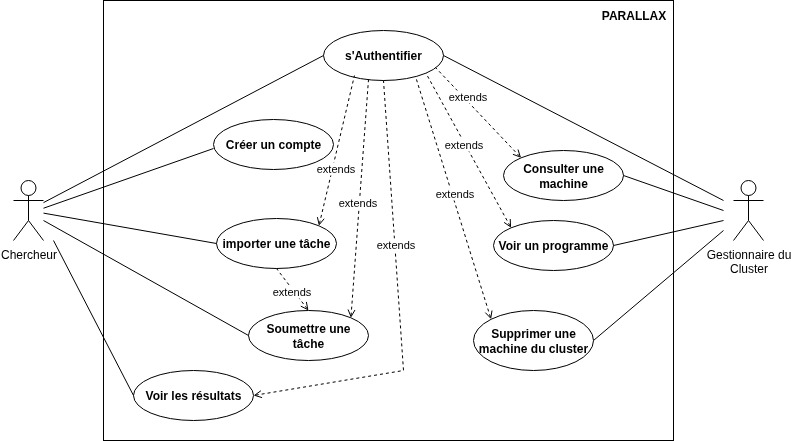
\includegraphics[width=\textwidth,height=\textheight,keepaspectratio]{images/Diagramme UC.jpg.jpeg}
    \caption{Diagramme de cas d'utilisation}
    \label{fig:use_case}
\end{figure}

\clearpage

\begin{table}[H]
\centering
\renewcommand{\arraystretch}{1.3}

\begin{tabular}{|p{4cm}|p{11cm}|}
\hline

\textbf{Objectif} & Accéder aux fonctionnalités du système \\ 
\hline

\textbf{Acteur(s)} & Chercheur, Gestionnaire du cluster \\ 
\hline

\textbf{Pré-condition} & Aucune \\ 
\hline

\textbf{Scénario nominal} & 
\begin{enumerate}
    \item L'acteur entre ses informations d'identification dans le système.
    \item Le système vérifie l'exactitude des informations.
    \item Les informations sont correctes, le système accorde l'accès aux fonctionnalités correspondantes au statut de l'utilisateur.
\end{enumerate} \\ 
\hline

\textbf{Scénarios alternatifs} & 
\begin{itemize}
    \item \textbf{A1 : Erreur de saisie} — Le système informe l'utilisateur et demande de nouvelles informations.
    \item \textbf{A2 : Erreur de connexion à la base de données} — Le système renvoie un message d'erreur.
\end{itemize} \\ 
\hline

\textbf{Post-condition} & Accès aux fonctionnalités liées au statut de l'utilisateur \\ 
\hline

\end{tabular}

\caption{Cas d’utilisation : Authentification}
\label{tab:authentification}
\end{table}


\begin{table}[H]
\centering
\renewcommand{\arraystretch}{1.3}

\begin{tabular}{|p{4cm}|p{11cm}|}
\hline

\textbf{Objectif} & Créer un compte utilisateur \\ 
\hline

\textbf{Acteur(s)} & Chercheur \\ 
\hline

\textbf{Pré-condition} & Être authentifié \\ 
\hline

\textbf{Scénario nominal} & 
\begin{enumerate}
    \item L'acteur entre ses informations dans le formulaire et le soumet au système.
    \item Le système vérifie l'exactitude des informations.
    \item Le système sauvegarde les informations et renvoie un message de succès.
\end{enumerate} \\ 
\hline

\textbf{Scénarios alternatifs} & 
\begin{itemize}
    \item \textbf{A1 : Erreur de saisie} — Le système demande à l'utilisateur de ressaisir ses informations.
    \item \textbf{A2 : Erreur de connexion à la base de données} — Le système renvoie un message d'erreur.
\end{itemize} \\ 
\hline

\textbf{Post-condition} & Création du compte utilisateur \\ 
\hline

\end{tabular}

\caption{Cas d’utilisation : Création de compte}
\label{tab:create_account}
\end{table}


\begin{table}[H]
\centering
\renewcommand{\arraystretch}{1.3}

\begin{tabular}{|p{4cm}|p{11cm}|}
\hline

\textbf{Objectif} & Importer une tâche annotée \\ 
\hline

\textbf{Acteur(s)} & Chercheur \\ 
\hline

\textbf{Pré-condition} & Être authentifié \\ 
\hline

\textbf{Scénario nominal} & 
\begin{enumerate}
    \item L'utilisateur clique sur l'option d'importation d'une tâche.
    \item Le système lui permet de sélectionner le dossier ou fichier annoté via un sélecteur de ressources.
    \item L'utilisateur sélectionne et valide.
    \item La tâche est enregistrée dans le système.
\end{enumerate} \\ 
\hline

\textbf{Scénarios alternatifs} & 
\begin{itemize}
    \item \textbf{A1 : Document invalide} — Le système annule l'importation et renvoie un message d'erreur.
\end{itemize} \\ 
\hline

\textbf{Post-condition} & Dossier / fichier importé dans le système \\ 
\hline

\end{tabular}

\caption{Cas d’utilisation : Importation d’une tâche}
\label{tab:import_task}
\end{table}



\begin{table}[H]
\centering
\renewcommand{\arraystretch}{1.3}

\begin{tabular}{|p{4cm}|p{11cm}|}
\hline

\textbf{Objectif} & Soumettre une tâche pour son exécution \\ 
\hline

\textbf{Acteur(s)} & Chercheur \\ 
\hline

\textbf{Pré-condition} & La tâche a été importée et le chercheur est authentifié \\ 
\hline

\textbf{Scénario nominal} & 
\begin{enumerate}
    \item L'utilisateur sélectionne la tâche à soumettre et valide.
    \item Le Master, grâce aux annotations, découpe et distribue la tâche à exécuter.
    \item Les Workers exécutent la tâche et renvoient les résultats au Master pour recomposition.
    \item Le Master recompose et renvoie le résultat à l'utilisateur.
\end{enumerate} \\ 
\hline

\textbf{Scénarios alternatifs} & 
\begin{itemize}
    \item \textbf{A1 : Erreur de connexion} — Un message d'erreur de connexion est renvoyé à l'utilisateur.
    \item \textbf{A2 : Dossier/fichier mal annoté} — Le système renvoie un message d'erreur d'annotation.
\end{itemize} \\ 
\hline

\textbf{Post-condition} & Le résultat de l'exécution est renvoyé à l'utilisateur \\ 
\hline

\end{tabular}

\caption{Cas d’utilisation : Soumission d’une tâche}
\label{tab:submit_task}
\end{table}



\begin{table}[H]
\centering
\renewcommand{\arraystretch}{1.3}

\begin{tabular}{|p{4cm}|p{11cm}|}
\hline

\textbf{Objectif} & Permettre à l'utilisateur de consulter les résultats de ses tâches exécutées \\ 
\hline

\textbf{Acteur(s)} & Chercheur \\ 
\hline

\textbf{Pré-condition} & Être authentifié \\ 
\hline

\textbf{Scénario nominal} & 
\begin{enumerate}
    \item L'utilisateur sélectionne le menu des résultats.
    \item Le système affiche les résultats et les détails d'exécution (durée, date, etc.).
\end{enumerate} \\ 
\hline

\textbf{Scénarios alternatifs} & 
\begin{itemize}
    \item \textbf{A1 : Aucun résultat} — Le système affiche un message indiquant l'absence de résultats.
    \item \textbf{A2 : Erreur de récupération} — Un message d'erreur est renvoyé à l'utilisateur.
\end{itemize} \\ 
\hline

\textbf{Post-condition} & Les résultats sont affichés à l'utilisateur \\ 
\hline

\end{tabular}

\caption{Cas d’utilisation : Consultation des résultats}
\label{tab:view_results}
\end{table}



\begin{table}[H]
\centering
\renewcommand{\arraystretch}{1.3}

\begin{tabular}{|p{4cm}|p{11cm}|}
\hline

\textbf{Objectif} & Consulter l'état d'une machine du cluster \\ 
\hline

\textbf{Acteur(s)} & Gestionnaire du cluster \\ 
\hline

\textbf{Pré-condition} & Être authentifié \\ 
\hline

\textbf{Scénario nominal} & 
\begin{enumerate}
    \item L'utilisateur sélectionne l'option de consultation des machines.
    \item Le système affiche la liste des machines du cluster.
    \item L'utilisateur sélectionne la machine souhaitée.
    \item Le système affiche les détails de la machine sélectionnée.
\end{enumerate} \\ 
\hline

\textbf{Scénarios alternatifs} & 
\begin{itemize}
    \item \textbf{A1 : Machine indisponible} — Le système affiche un message d'erreur d'accessibilité.
    \item \textbf{A2 : Liste vide} — Le système indique qu'aucune machine n'est disponible.
\end{itemize} \\ 
\hline

\textbf{Post-condition} & Les détails de la machine sont affichés \\ 
\hline

\end{tabular}

\caption{Cas d’utilisation : Consultation d’une machine}
\label{tab:view_machine}
\end{table}



\begin{table}[H]
\centering
\renewcommand{\arraystretch}{1.3}

\begin{tabular}{|p{4cm}|p{11cm}|}
\hline

\textbf{Objectif} & Déconnecter une machine du cluster \\ 
\hline

\textbf{Acteur(s)} & Gestionnaire du cluster \\ 
\hline

\textbf{Pré-condition} & Être authentifié \\ 
\hline

\textbf{Scénario nominal} & 
\begin{enumerate}
    \item L'utilisateur sélectionne la machine à arrêter dans la liste.
    \item L'utilisateur déclenche la commande d'arrêt distant.
    \item Le système demande à l'agent sur la machine d'exécuter la commande d'arrêt.
    \item L'état de la machine est mis à jour sur l'interface pour confirmer l'arrêt.
\end{enumerate} \\ 
\hline

\textbf{Scénarios alternatifs} & 
\begin{itemize}
    \item \textbf{A1 : Échec de communication} — Le système affiche un message d'échec et propose de réessayer.
    \item \textbf{A2 : Refus de confirmation} — L'utilisateur annule, la procédure est abandonnée sans modification.
    \item \textbf{A3 : Machine en cours d'exécution critique} — Le système demande une confirmation supplémentaire ou bloque l'action.
\end{itemize} \\ 
\hline

\textbf{Post-condition} & La machine est arrêtée (déconnectée du cluster) \\ 
\hline

\end{tabular}

\caption{Cas d’utilisation : Suppression d’une machine du cluster}
\label{tab:delete_machine}
\end{table}


\begin{table}[H]
\centering
\renewcommand{\arraystretch}{1.3}

\begin{tabular}{|p{4cm}|p{11cm}|}
\hline

\textbf{Objectif} & Voir en temps réel l'état d'un programme en cours d'exécution \\ 
\hline

\textbf{Acteur(s)} & Gestionnaire du cluster \\ 
\hline

\textbf{Pré-condition} & Être authentifié \\ 
\hline

\textbf{Scénario nominal} & 
\begin{enumerate}
    \item L'utilisateur sélectionne l'option de consultation des tâches en cours.
    \item Le système affiche la liste des tâches actives.
    \item L'utilisateur sélectionne la tâche souhaitée.
    \item Le système affiche les détails d'exécution (machines impliquées, pourcentage d'avancement, etc.).
\end{enumerate} \\ 
\hline

\textbf{Scénarios alternatifs} & 
\begin{itemize}
    \item \textbf{A1 : Aucune tâche en cours} — Le système affiche un message d'absence de tâches actives.
    \item \textbf{A2 : Erreur de récupération} — Le système affiche un message d'erreur et propose de réessayer.
\end{itemize} \\ 
\hline

\textbf{Post-condition} & Les détails d'exécution de la tâche sont affichés \\ 
\hline

\end{tabular}

\caption{Cas d’utilisation : Consultation d’un programme en cours d’exécution}
\label{tab:view_program}
\end{table}
% ------------------------------------------------------------

% ------------------------------------------------------------
\subsubsection{Interaction Systemes}
\subsubsection*{Presentation de Sequences Systeme}
\begin{figure}[H]
    \centering
    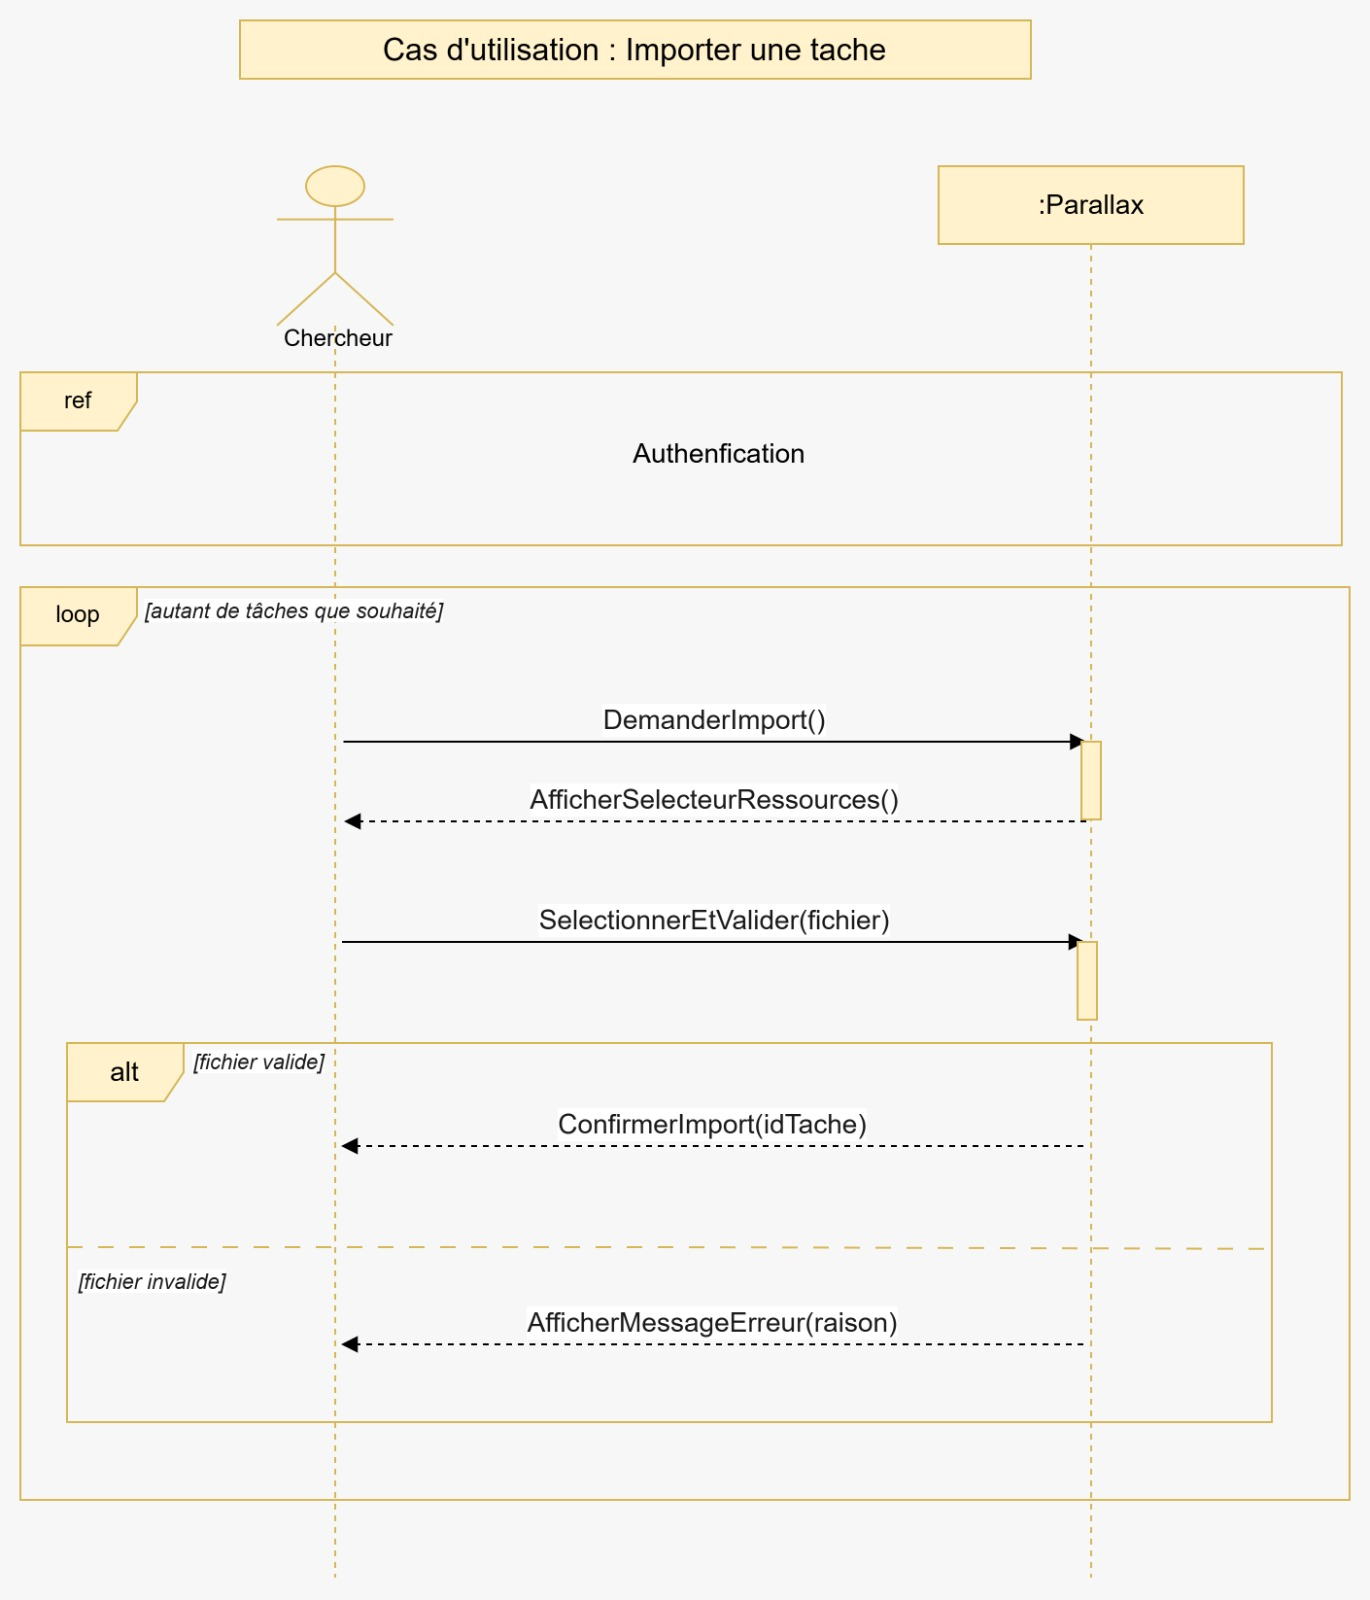
\includegraphics[width=1\textwidth]{images/diagramme de sequences - importer une tache - parallax .jpeg}
    \caption{Diagramme de séquences système — Importer une tâche}
    \label{fig:seq_import}
\end{figure}

\begin{figure}[H]
    \centering
    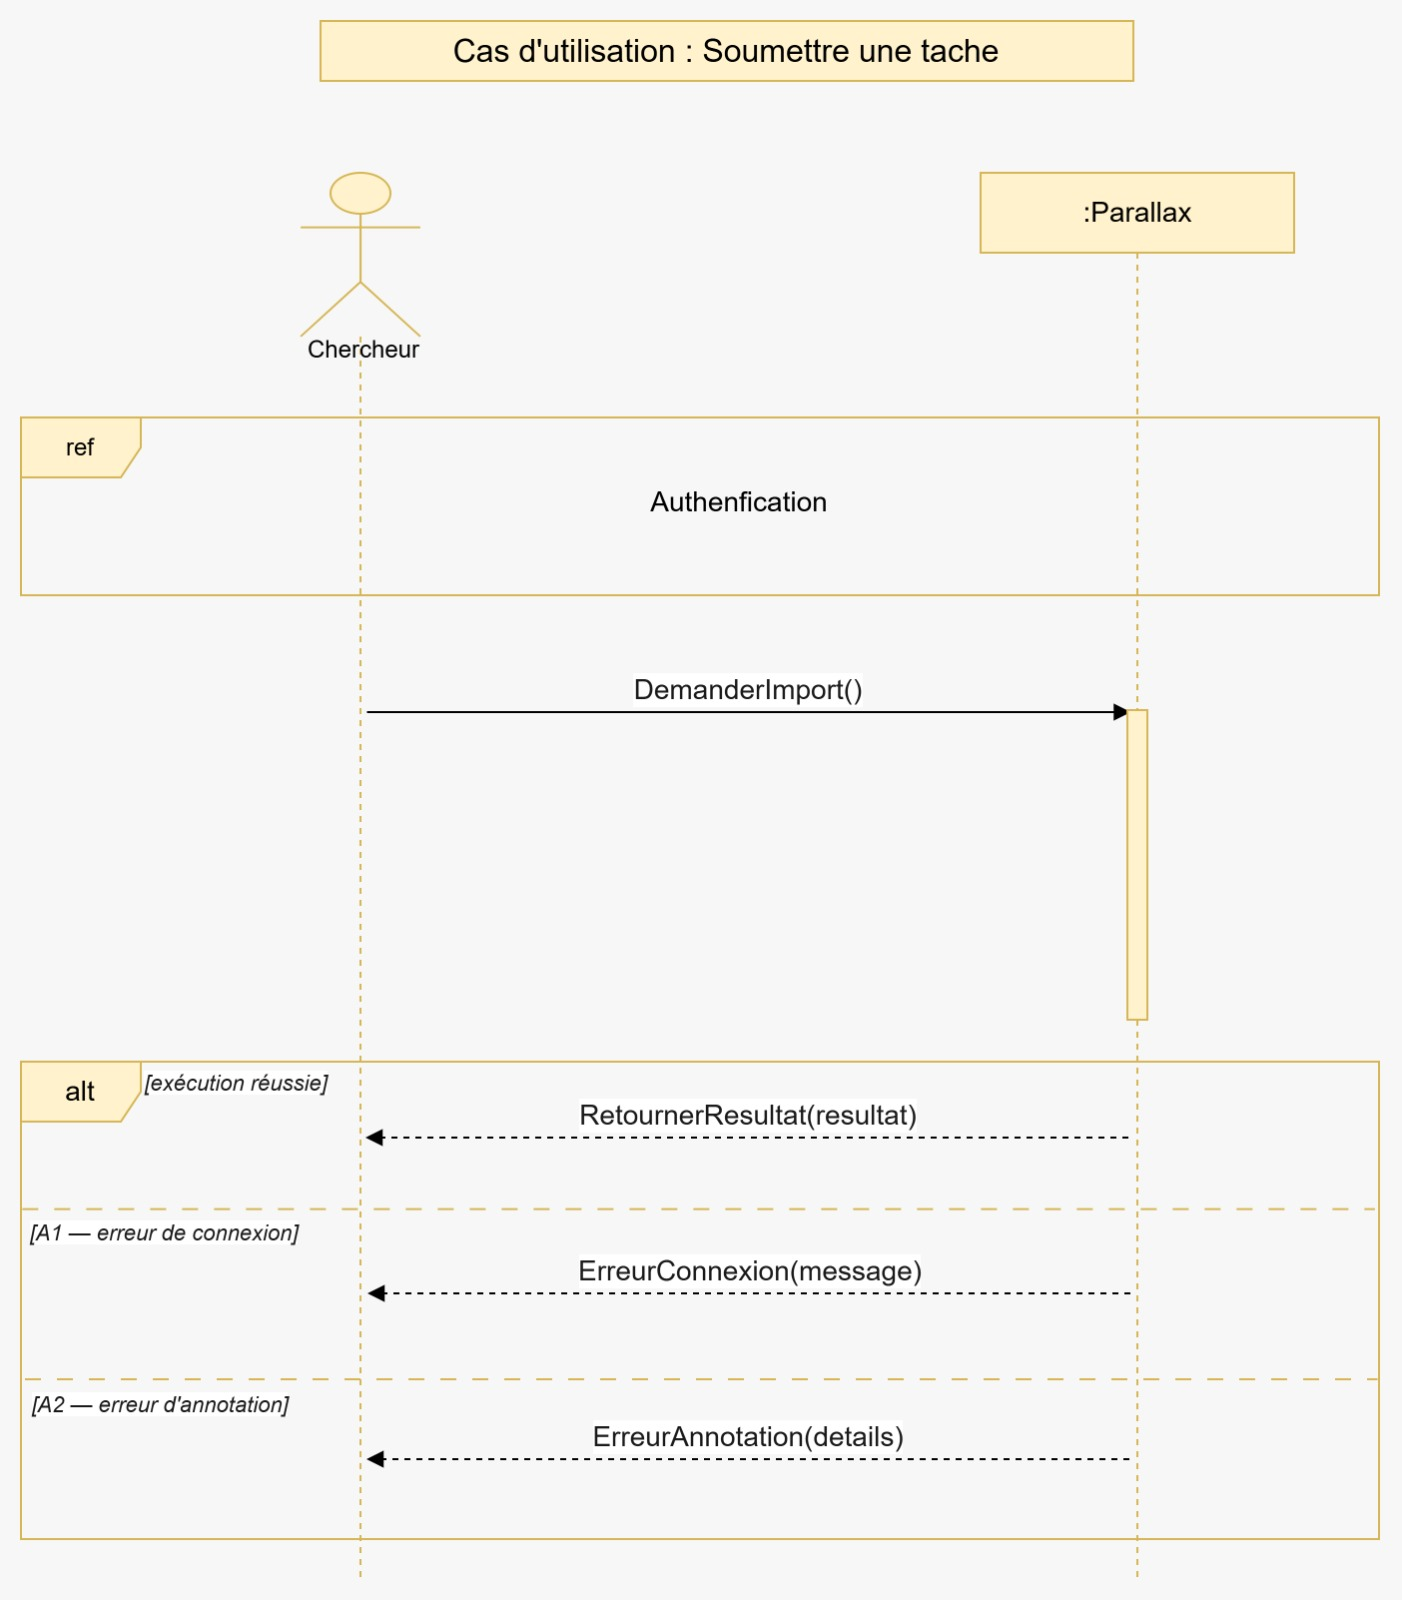
\includegraphics[width=1\textwidth]{images/diagramme de sequence - soumettre une tache- parallax.jpeg}
    \caption{Diagramme de séquences système — Soumettre une tâche}
    \label{fig:seq_soumettre}
\end{figure}

\begin{figure}[H]
    \centering
    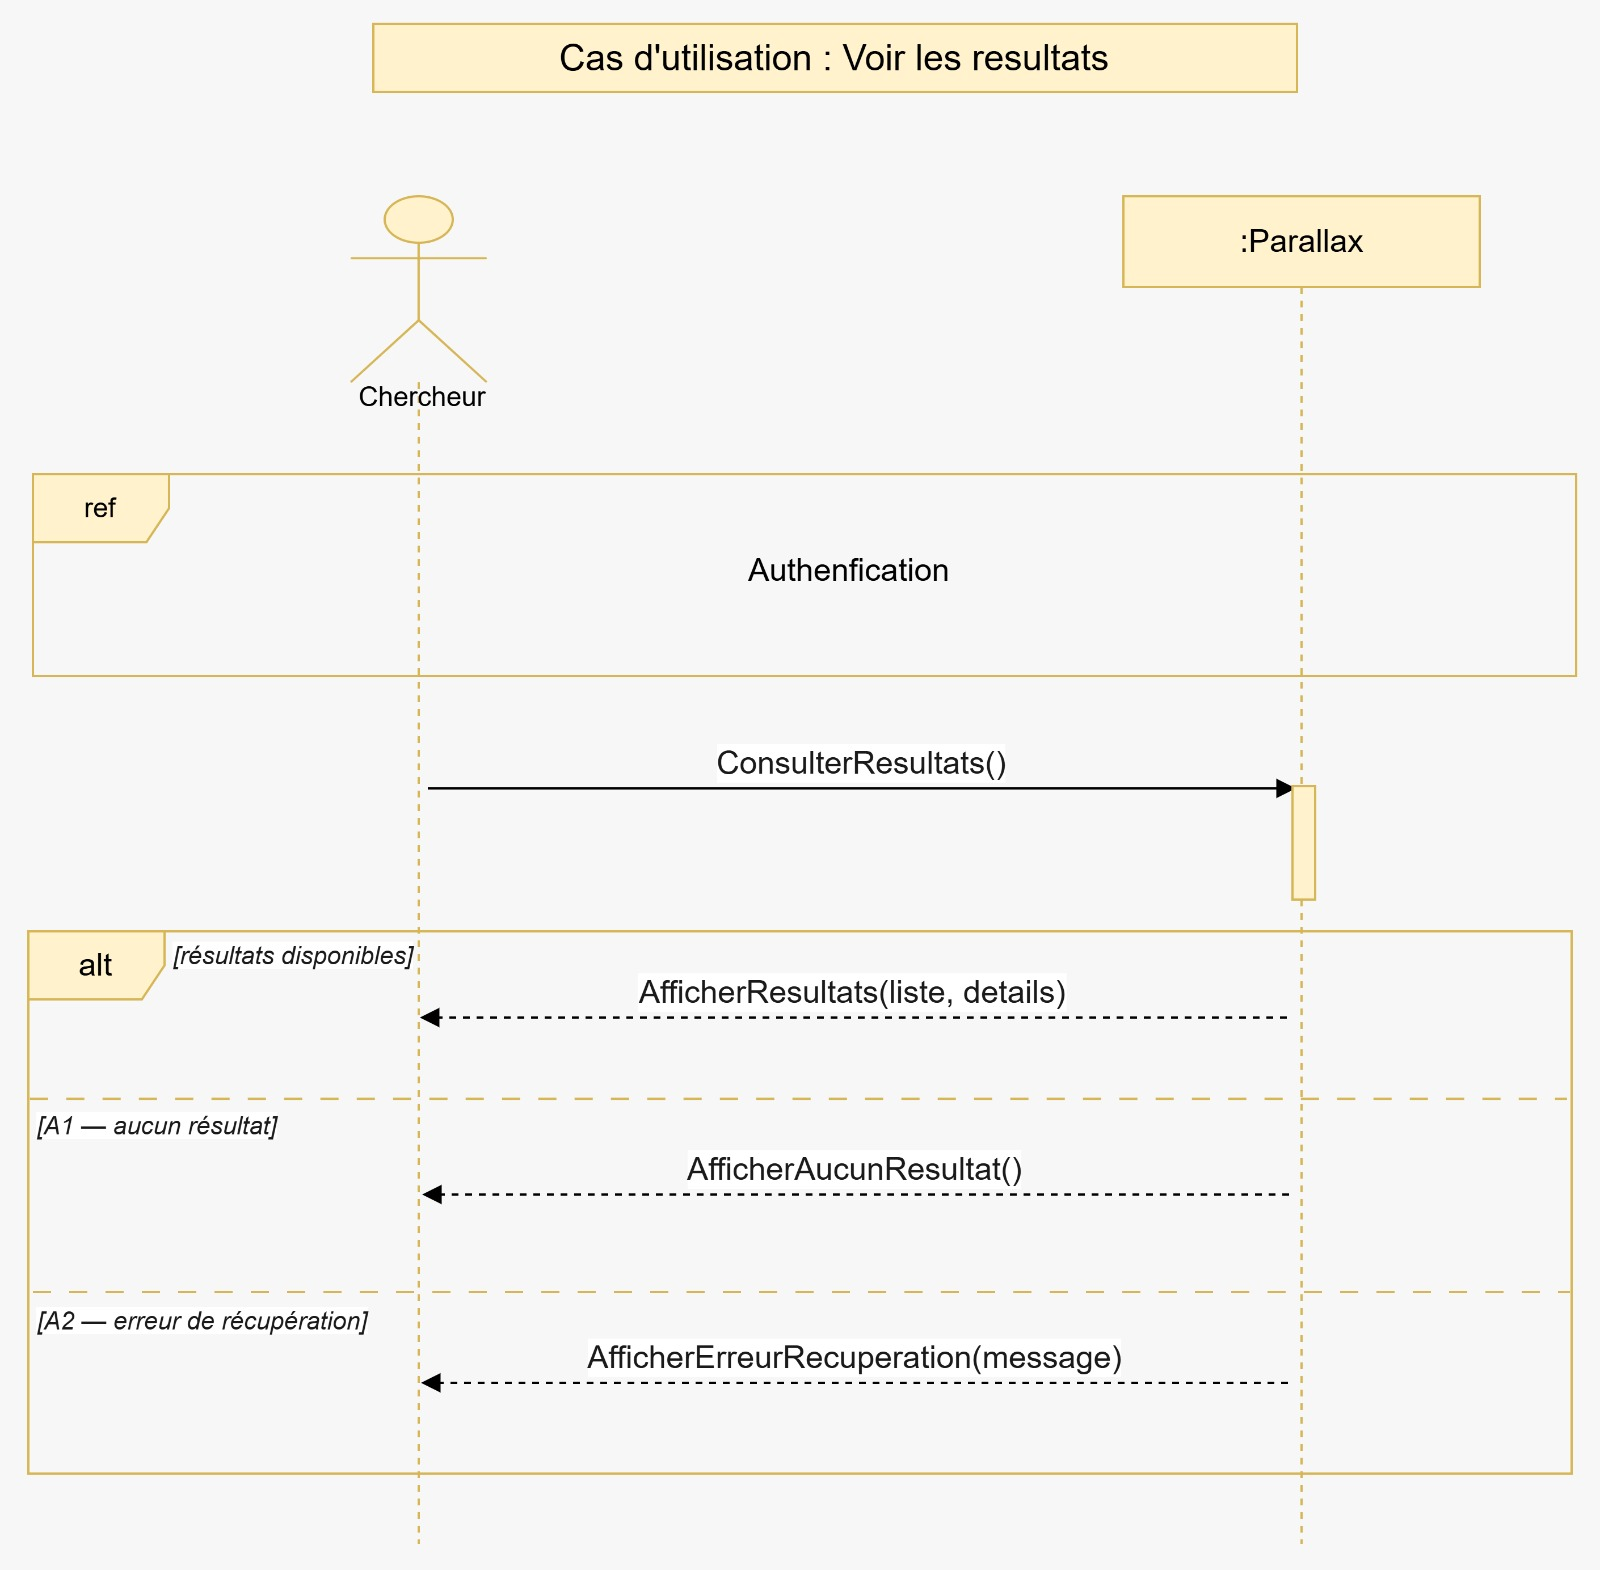
\includegraphics[width=1\textwidth]{images/sequence systeme - voir les resultats.jpeg}
    \caption{Diagramme de séquences système — Voir les résultats}
    \label{fig:seq_resultats}
\end{figure}

\begin{figure}[H]
    \centering
    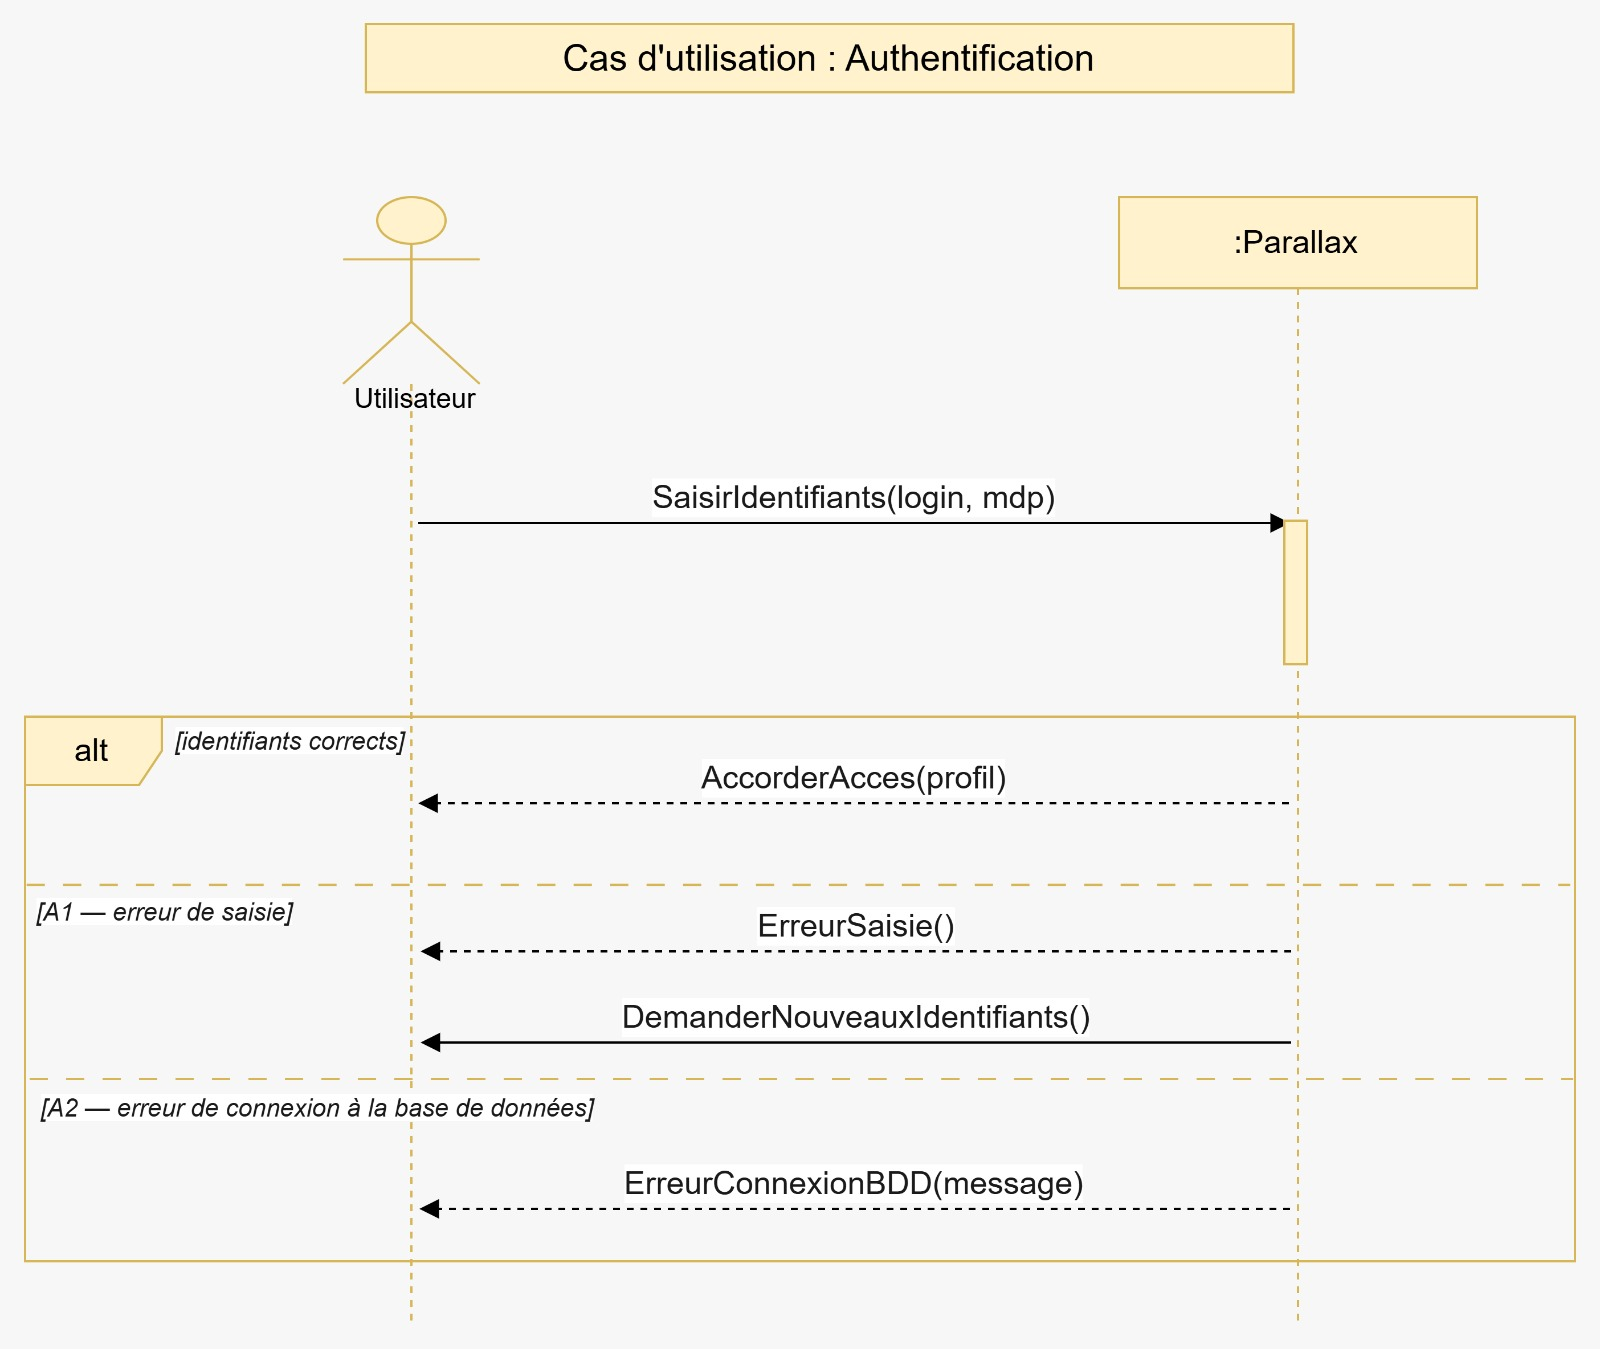
\includegraphics[width=1\textwidth]{images/diagramme de sequences systeme - authhentification - parallax.jpeg}
    \caption{Diagramme de séquences système — Authentification}
    \label{fig:seq_auth}
\end{figure}

\begin{figure}[H]
    \centering
    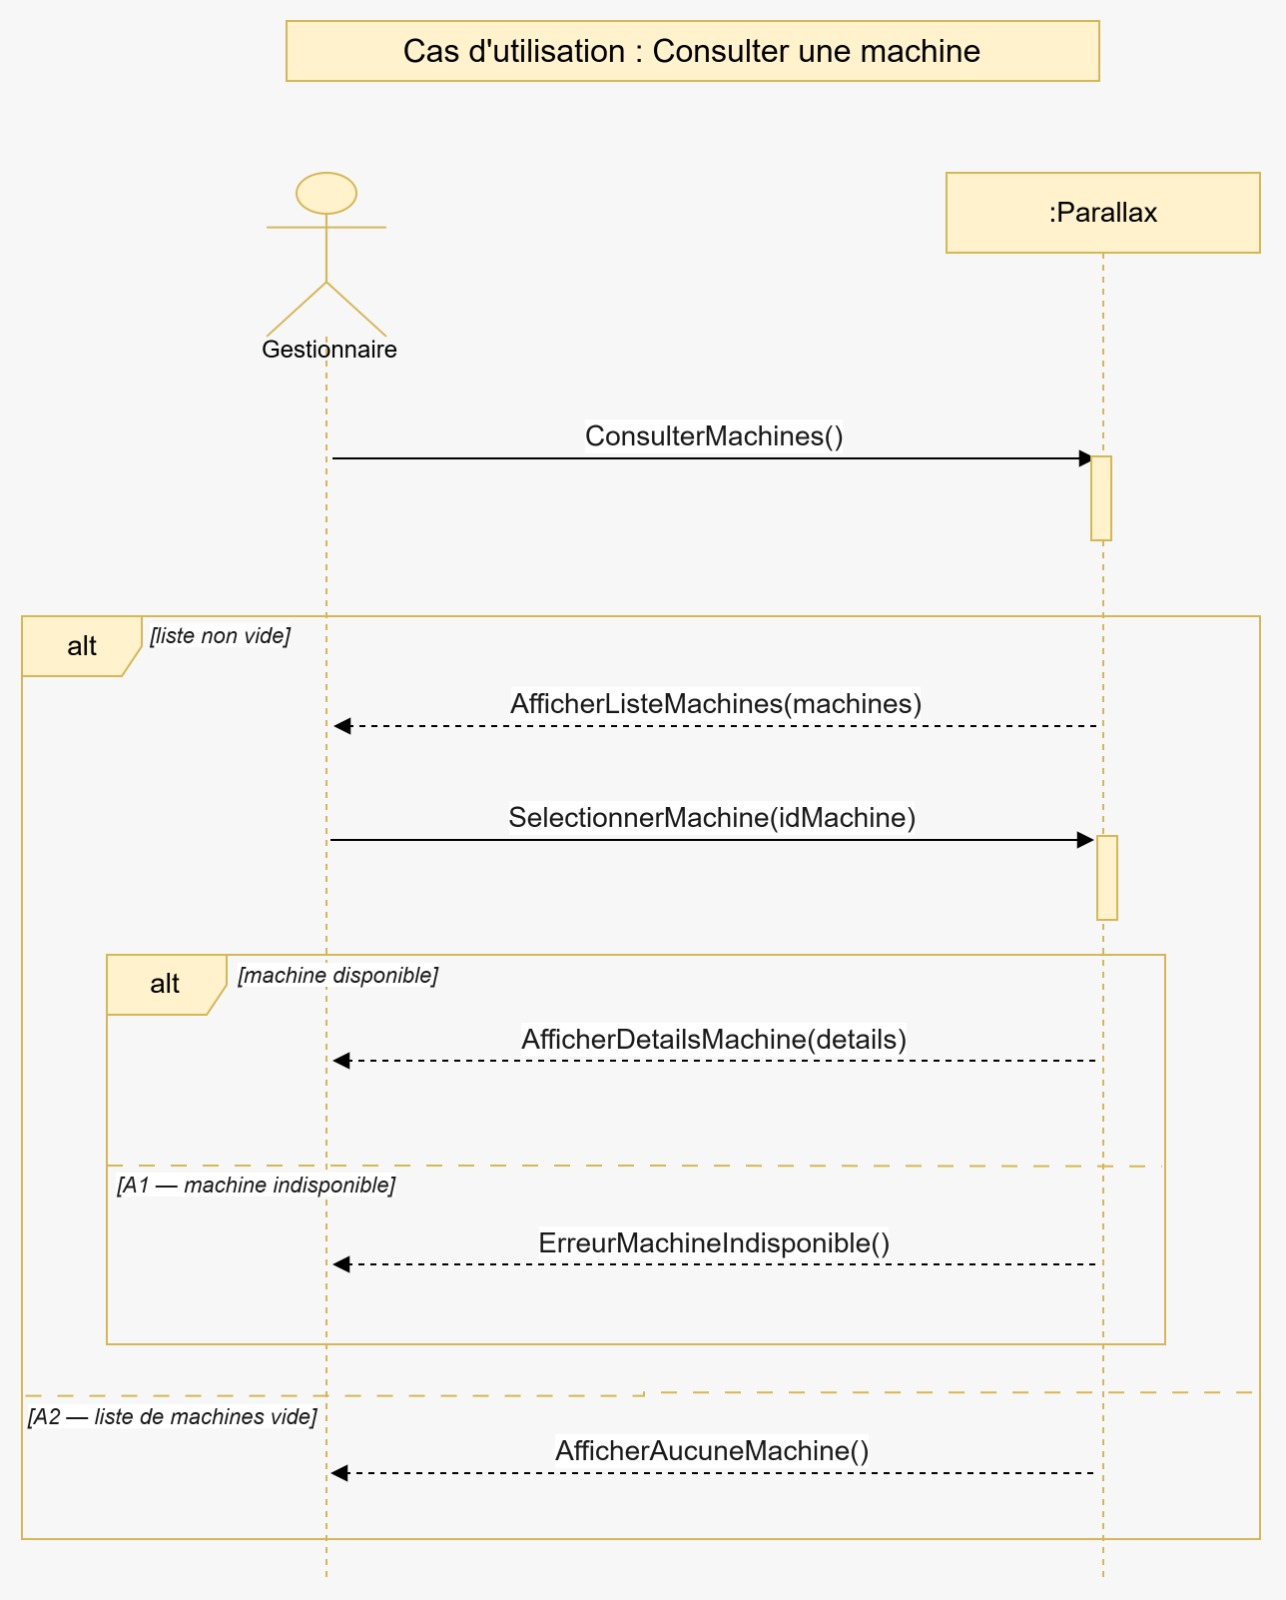
\includegraphics[width=1\textwidth]{images/sequence systeme - consulter une machine.jpeg}
    \caption{Diagramme de séquences système — Consulter une machine}
    \label{fig:seq_machine}
\end{figure}
\subsubsection*{Presenations des Classes Metiers}


\subsubsection{Presentation des Etats Transition}

\section{Conception}


Notre système permet aux chercheurs d’effectuer des calculs de simulation en s’appuyant sur des machines récupérées au sein de l’ENSPY. Ces machines sont mises en réseau et combinées afin de résoudre efficacement les problèmes soumis par les chercheurs.

Le système offre la possibilité aux utilisateurs de soumettre leurs calculs à partir d’une machine dédiée. Les tâches sont ensuite découpées en sous-calculs et distribuées aux différentes machines du réseau. Chaque machine exécute sa partie du calcul, puis renvoie les résultats à une machine centrale. Celle-ci se charge de les agréger afin de produire le résultat final.

Dans cette approche, chaque machine est considérée comme un \textbf{agent autonome}, ce qui permet de modéliser le système comme un \textbf{système multi-agents.}

\subsection{Modélisation agentique du système}

\subsubsection{Vue globale du SMA Parrallax}
Le fonctionnement global du système multi-agents Parrallax peut être résumé comme suit :
\begin{enumerate}
    \item Réception du calcul soumis par le chercheur ;
    \item Décomposition du calcul en sous-calculs ;
    \item Répartition des sous-calculs entre les agents ;
    \item Exécution des sous-calculs par les agents ;
    \item Retour des résultats partiels ;
    \item Recombinaison des résultats ;
    \item Production du résultat final.
\end{enumerate}

\subsubsection{Modélisation d’un agent}

\paragraph{Aspect physique}

Chaque machine $v \in V_M$ est caractérisée par un vecteur d’état décrivant ses différentes propriétés :

\[
X_v =
\begin{bmatrix}
ID_v \\
NET_v \\
COMPUTE_v \\
MEMORY_v \\
STORAGE_v \\
LOAD_v \\
RELIABILITY_v \\
STATE_v \\
SECURITY_v
\end{bmatrix}
\]

Les composantes de ce vecteur représentent les différentes dimensions du système :

\begin{itemize}
    \item[*] $ID_v = (\text{uuid}, \text{role}, \text{region})$ :
    \begin{itemize}
        \item[>] \textit{uuid} identifie de manière unique la machine ;
        \item[>] \textit{role} spécifie son rôle dans le système ;
        \item[>] \textit{region} indique sa localisation.
    \end{itemize}

    \item[*] $NET_v = (\text{ip}, \text{latency}, \text{bandwidth}_{in}, \text{bandwidth}_{out}, \text{jitter}, \text{loss})$ : paramètres caractérisant les performances réseau.

    \item[*] $COMPUTE_v = (\text{cpucores}, \text{cpufreq}, \text{gpu}, \text{flops})$ : capacités de calcul de la machine.

    \item[*] $MEMORY_v = (\text{ram}, \text{mem\_bandwidth})$ : ressources mémoire disponibles.

    \item[*] $STORAGE_v = (\text{disk}, \text{io})$ : capacités de stockage et performances d’entrée/sortie.

    \item[*] $LOAD_v = (\text{cpuusage}, \text{ramusage}, \text{queue})$ : niveau de charge courant de la machine.

    \item[*] $STATE_v = (\text{status}, \text{availability})$ : état opérationnel de la machine.

    \item[*] $RELIABILITY_v = (\text{uptime}, \text{failurerate})$ : indicateurs de fiabilité.

    \item[*] $SECURITY_v = (\text{auth}, \text{trust})$ : paramètres liés à la sécurité et à la confiance.
\end{itemize}
\paragraph{Aspect logique}

Le système est organisé autour de différents rôles fonctionnels. Un agent peut endosser un ou plusieurs de ces rôles selon les besoins du système. Ces rôles définissent les responsabilités et les interactions attendues, sans correspondre nécessairement à des entités distinctes.

\subsubsection{Rôles des agents}

Les rôles fonctionnels au sein du système sont les suivants :

\begin{enumerate}
    \item \textbf{Rôle de réception} : correspond à la prise en charge des calculs soumis via une interface utilisateur. Ce rôle implique l’entrée des requêtes dans le système.

    \item \textbf{Rôle de contrôle réseau} : assure la surveillance de l’état global du système et la collecte des informations de statut des composants.

    \item \textbf{Rôle de génération de sous-calculs} : consiste à décomposer un calcul global en unités plus petites et exploitables.

    \item \textbf{Rôle d’orchestration} : implique la répartition des sous-calculs en fonction des ressources disponibles et de l’état du système.

    \item \textbf{Rôle de synthèse} : consiste à agréger et recombiner les résultats partiels afin de produire un résultat final cohérent.

    \item \textbf{Rôle d’exécution} : correspond à la réalisation effective des calculs ou sous-calculs assignés.
\end{enumerate}

\subsubsection{Définition des agents du monde SMA\_PARALLAX}

Dans cette partie, nous décrivons les différents types d’agents du système SMA\_PARALLAX ainsi que leurs caractéristiques et comportements agentiques.

\begin{enumerate}

%------------------------------------------------
\item \textbf{Agent Master}

L’agent Master est responsable de la réception, de la gestion et de la coordination de l’exécution des tâches. Il constitue le point central du système.

\begin{itemize}
    \item [$\bullet$]\textbf{Environnement :} Interface utilisateur et système distribué.

    \item [$\bullet$]\textbf{Actions :}
    \begin{itemize}
        \item[$-$] \textbf{Réception des calculs :} Le nœud maître reçoit les requêtes de calcul soumises par les chercheurs via une interface.
        
\item[$-$] \textbf{Décomposition des tâches :} Il décompose un calcul global en plusieurs sous-calculs.
        
\item[$-$] \textbf{Réception des états du cluster :} Il reçoit, via le contrôleur, les informations d’état des différentes machines (CPU, RAM, latence) afin d’avoir une vision globale actualisée du cluster.
        
\item[$-$] \textbf{Distribution des sous-calculs :} Il répartit les sous-calculs entre les agents Worker disponibles en tenant compte de leurs capacités et de leur état.
        
\item[$-$] \textbf{Réception des résultats :} Il reçoit les résultats partiels provenant des Workers.
        
\item[$-$] \textbf{Agrégation des résultats :} Il combine les résultats des sous-calculs afin de produire le résultat final.
        
\item[$-$] \textbf{Exécution locale (optionnelle) :} Il peut exécuter certaines tâches légères localement.
        
\item[$-$] \textbf{Observation du système :} Il surveille l’état des autres machines et agents.
        
\item[$-$] \textbf{Diffusion de son état :} Il communique son état au reste du système lorsque nécessaire.
    \end{itemize}
\end{itemize}

%------------------------------------------------
\item \textbf{Agent Worker}

L’agent Worker est responsable de l’exécution des sous-tâches qui lui sont assignées. Il agit comme unité de calcul dans le système distribué.

\begin{itemize}
    \item [$\bullet$]\textbf{Environnement :} Réseau distribué de machines interconnectées.

    \item [$\bullet$]\textbf{Actions :}
    \begin{itemize}
        \item[$-$] \textbf{Échange de messages :} Les Workers peuvent communiquer avec les autres nœuds du système.
        
        \item[$-$] \textbf{Réception des sous-calculs :} Ils reçoivent les tâches envoyées par l’agent Master.
        
        \item [$-$]\textbf{Exécution des sous-calculs :} Ils exécutent localement les tâches assignées.
        
        \item [$-$]\textbf{Retour des résultats :} Ils renvoient les résultats au Master après exécution.
        
        \item [$-$]\textbf{Diffusion de l’état :} Ils envoient périodiquement leur état (charge, disponibilité, performance).
    \end{itemize}
\end{itemize}

%------------------------------------------------
\item \textbf{Agent Contrôleur}

L’agent Contrôleur est chargé de maintenir une vue globale cohérente de l’état du système, notamment en ce qui concerne la présence, la disponibilité et les caractéristiques des agents.

\begin{itemize}
    \item[$\bullet$] \textbf{Environnement :} Ensemble des agents du réseau distribué.

    \item [$\bullet$]\textbf{Actions :}
    \begin{itemize}
       \item[$-$] \textbf{Détection des problèmes :} Il notifie l’agent Master en cas de panne ou de défaillance d’un nœud. En cas de défaillance du Master lui-même, il informe également les autres nœuds du cluster afin de déclencher un mécanisme approprié(où celui du vote est compris) et assurer la continuité du système.
        
        \item [$-$]\textbf{Réception des états :} Il collecte les informations d’état des différentes machines.
        
        \item[$-$] \textbf{Enregistrement des nœuds :} Il intègre les nouveaux nœuds dans le système.
    \end{itemize}
\end{itemize}

\end{enumerate}


\begin{table}[H]
\centering
\renewcommand{\arraystretch}{1.3}
\begin{tabular}{|c|p{3cm}|p{4cm}|p{3cm}|p{2cm}|p{2cm}|}
\hline
\textbf{N°} & \textbf{Nom de l’action} & \textbf{Commentaire} & \textbf{Rôle d’agent} & \textbf{Données d’entrée} & \textbf{Données de sortie} \\
\hline

1 & Réception des calculs & Prise en charge des requêtes utilisateur & Réception (Master) & Requête utilisateur & Tâche globale \\
\hline

2 & Décomposition des tâches & Division du calcul global en sous-calculs & Génération (Master) & Tâche globale & Sous-calculs \\
\hline

3 & Distribution des sous-calculs & Allocation des tâches aux Workers & Orchestration (Master) & Sous-calculs + état des Workers & Tâches assignées \\
\hline

4 & Réception des sous-calculs & Réception des tâches envoyées par le Master & Exécution (Worker) & Sous-calculs & Tâches locales \\
\hline

5 & Exécution des sous-calculs & Calcul effectif des tâches & Exécution (Worker) & Tâches locales & Résultats partiels \\
\hline

6 & Retour des résultats & Envoi des résultats vers le Master & Exécution (Worker) & Résultats partiels & Résultats transmis \\
\hline

7 & Agrégation des résultats & Combinaison des résultats partiels & Synthèse (Master) & Résultats partiels & Résultat final \\
\hline

8 & Observation du système & Surveillance des ressources et états & Contrôle réseau (Master) & États des agents & Vue système \\
\hline

9 & Diffusion de l’état Worker & Communication de la charge et disponibilité & Contrôle réseau (Worker) & État local & Infos d’état \\
\hline

10 & Réception des états & Collecte des infos système & Contrôle réseau (Contrôleur) & Infos d’état & Base de données état \\
\hline

11 & Détection des problèmes & Identification des pannes & Contrôle réseau (Contrôleur) & États système & Alertes \\
\hline

12 & Notification des défaillances & Alerte envoyée au Master & Contrôle réseau (Contrôleur) & Alertes & Notification \\
\hline

13 & Enregistrement des nœuds & Ajout de nouveaux agents & Contrôle réseau (Contrôleur) & Infos nouveau nœud & Nœud enregistré \\
\hline

\end{tabular}
\caption{Table des actions du système SMA\_PARALLAX}
\end{table}


\subsection{Interactions entre agents}

Dans un système multi-agents distribué tel que \textbf{SMA\_PARALLAX}, les interactions entre agents constituent un élément central assurant la coordination, la cohérence et l’efficacité globale du système. 

Ces interactions reposent principalement sur des mécanismes d’échange de messages et de partage d’informations d’état, permettant aux différents agents d’adapter dynamiquement leur comportement en fonction du contexte d’exécution. Chaque rôle fonctionnel (réception, génération, orchestration, exécution, synthèse et contrôle) n’agit pas de manière isolée, mais s’inscrit dans une chaîne d’interactions structurée formant un pipeline de traitement distribué.

Ainsi, le flux global du système peut être décrit comme suit :
\begin{itemize}
    \item Une requête utilisateur est introduite dans le système via l’agent de réception.
    \item Cette requête est transformée en sous-tâches par l’agent générateur.
    \item Les sous-tâches sont ensuite distribuées de manière optimale par l’orchestrateur.
    \item Les agents d’exécution réalisent les calculs et produisent des résultats partiels.
    \item Enfin, l’agent de synthèse agrège ces résultats pour produire une sortie finale cohérente.
\end{itemize}

Parallèlement à ce flux principal, des interactions transversales assurent la supervision du système, notamment via la collecte et la diffusion d’informations d’état entre agents.

Les figures suivantes illustrent les principales interactions entre les différents rôles du système :

\begin{figure}[H]
    \centering
    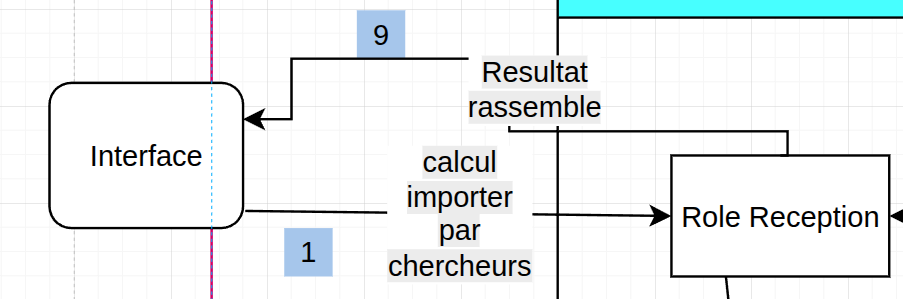
\includegraphics[width=0.5\linewidth]{image.png}
    \caption{Interaction entre le rôle de réception et son environnement}
    \label{fig:interaction_reception_env}
\end{figure}

Cette interaction met en évidence la phase d’entrée du système, où les requêtes utilisateur sont capturées et injectées dans le système multi-agents.

\begin{figure}[H]
    \centering
    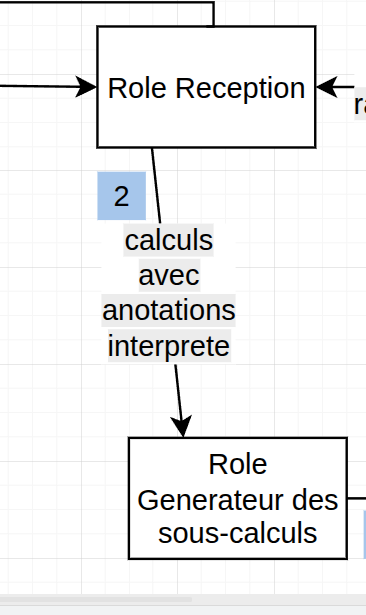
\includegraphics[width=0.5\linewidth]{image2.png}
    \caption{Interaction entre le réceptionniste et le générateur de sous-tâches}
    \label{fig:interaction_reception_generation}
\end{figure}

Cette étape correspond à la transmission de la tâche globale vers le module de décomposition.

\begin{figure}[H]
    \centering
    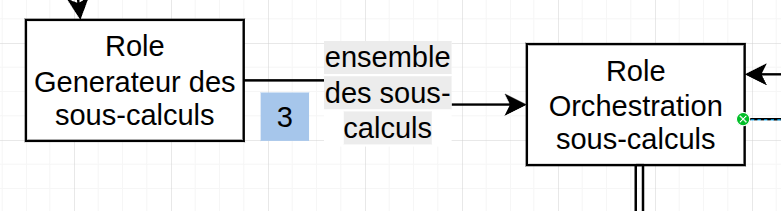
\includegraphics[width=0.5\linewidth]{image3.png}
    \caption{Interaction détaillée entre réception et génération des sous-calculs}
    \label{fig:interaction_detail_generation}
\end{figure}

Elle illustre plus finement le processus de partages des calculs en sous-calculs.

\begin{figure}[H]
    \centering
    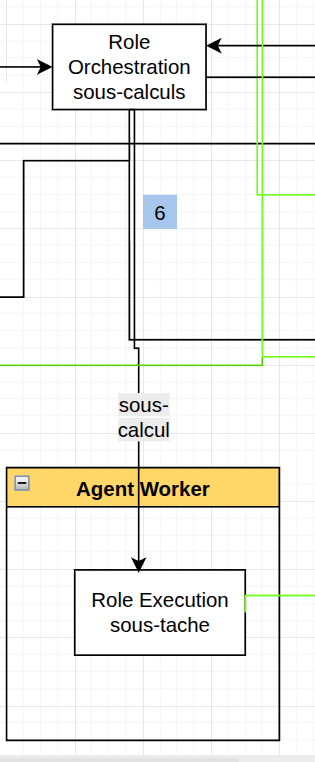
\includegraphics[width=0.5\linewidth]{image4.png}
    \caption{Interaction entre le générateur de sous-calculs et l’orchestrateur}
    \label{fig:interaction_generation_orchestration}
\end{figure}

Cette interaction met en évidence la phase de planification et d’allocation des ressources.

\begin{figure}[H]
    \centering
    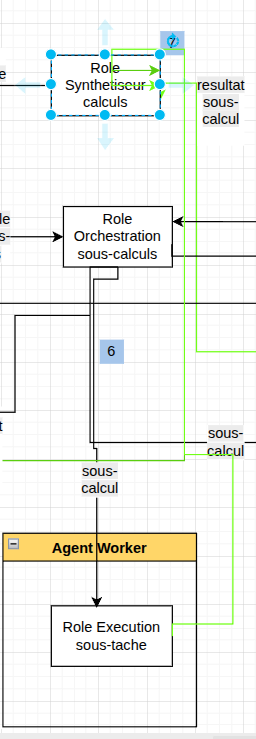
\includegraphics[width=0.5\linewidth]{image5.png}
    \caption{Interaction entre les agents d’exécution et le synthétiseur}
    \label{fig:interaction_execution_synthese}
\end{figure}

Elle représente le retour des résultats partiels vers le module de synthèse.

\begin{figure}[H]
    \centering
    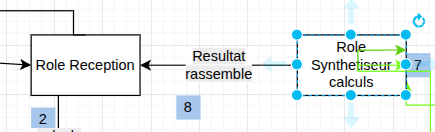
\includegraphics[width=0.5\linewidth]{image6.png}
    \caption{Interaction entre le synthétiseur et le réceptionniste}
    \label{fig:interaction_synthese_reception}
\end{figure}

Cette dernière interaction boucle le cycle en transmettant le résultat final vers l’interface utilisateur.

\bigskip


\subsubsection{Table des événements du système}

Dans le système SMA\_PARALLAX, le fonctionnement repose sur un ensemble d’événements discrets déclenchant les actions des agents. Chaque événement correspond à une transition dans le cycle de traitement distribué et peut être associé à un ou plusieurs rôles agentiques.

Le tableau suivant présente les principaux événements identifiés dans le système ainsi que leur description :

\begin{table}[H]
\centering
\renewcommand{\arraystretch}{1.3}
\begin{tabular}{|c|p{4cm}|p{9cm}|}
\hline
\textbf{N°} & \textbf{Nom de l’événement} & \textbf{Description} \\
\hline

E1 & Soumission de calcul & Un utilisateur soumet une requête de calcul via l’interface du système. Cet événement déclenche l’activation de l’agent de réception. \\
\hline

E2 & Réception de tâche globale & L’agent Master reçoit et valide la tâche globale à traiter. \\
\hline

E3 & Décomposition déclenchée & La tâche globale est transformée en sous-calculs exploitables par les agents Worker. \\
\hline

E4 & Disponibilité des ressources & Les informations sur l’état des Workers (charge, disponibilité) sont utilisées pour planifier la distribution. \\
\hline

E5 & Allocation des sous-calculs & Les sous-tâches sont assignées aux agents Worker selon une stratégie d’orchestration. \\
\hline

E6 & Réception d’un sous-calcul & Un agent Worker reçoit une tâche à exécuter. \\
\hline

E7 & Début d’exécution & Le Worker commence le traitement du sous-calcul assigné. \\
\hline

E8 & Fin d’exécution & Le Worker termine l’exécution du sous-calcul et produit un résultat partiel. \\
\hline

E9 & Envoi du résultat partiel & Le résultat calculé est transmis au Master. \\
\hline

E10 & Réception des résultats partiels & Le Master collecte les résultats provenant de plusieurs Workers. \\
\hline

E11 & Agrégation des résultats & Les résultats partiels sont combinés pour produire un résultat global cohérent. \\
\hline

E12 & Production du résultat final & Le résultat final est généré et prêt à être renvoyé à l’utilisateur. \\
\hline

E13 & Diffusion d’état (Worker) & Les Workers envoient périodiquement leurs informations d’état (charge, disponibilité). \\
\hline

E14 & Collecte des états & L’agent Contrôleur centralise les informations provenant des différents agents. \\
\hline

E15 & Détection de défaillance & Une anomalie ou panne d’un nœud est détectée dans le système. \\
\hline

E16 & Notification de défaillance & Une alerte est envoyée au Master pour adapter l’orchestration. \\
\hline

E17 & Enregistrement d’un nouveau nœud & Un nouvel agent rejoint le système et est intégré dans l’environnement distribué. \\
\hline

\end{tabular}
\caption{Table des événements du système SMA\_PARALLAX}
\end{table}


\subsection{Architecture Agentique}

Cette section présente l’architecture agentique du système PARALLAX. Elle décrit l’organisation des différents agents, leurs interactions ainsi que leur rôle dans l’exécution distribuée des tâches. Cette architecture permet de structurer le système en entités autonomes capables de coopérer pour assurer la scalabilité, la robustesse et l’efficacité du calcul distribué.

\begin{figure}[H]
    \centering
    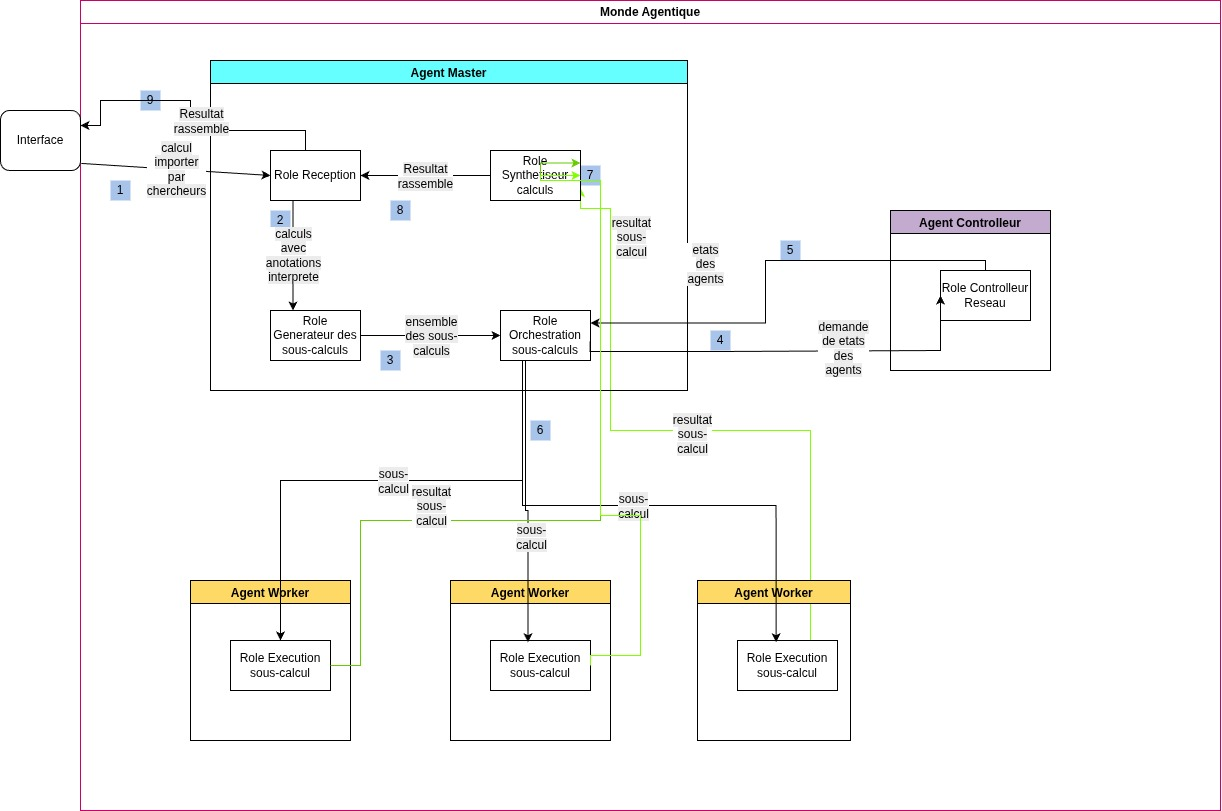
\includegraphics[width=1.25\linewidth]{Architecture_agentique (2).jpg}
    \caption{Architecture Agentique}
    \label{fig:placeholder}
\end{figure}
\section{Presentation des Algorithmes Cles}
\subsection{Présentation de l’algorithme d’inscription d’un nouveau nœud}

\paragraph{Principe}
L’inscription d’un nouveau nœud dans le cluster repose sur un processus d’auto-intégration dans lequel le nœud obtient une adresse réseau, génère une identité unique et se déclare auprès du contrôleur. Une fois validé, il est intégré au système et devient opérationnel pour participer aux calculs distribués.

\paragraph{Entrée}
\begin{itemize}
    \item[$\bullet$] Nœud $N$ rejoignant le réseau
    \item[$\bullet$] Accès au service DHCP
    \item[$\bullet$]Accès au canal de diffusion réseau (broadcast)
    \item [$\bullet$]Présence du contrôleur du cluster
\end{itemize}

\paragraph{Algorithme}

\begin{algorithm}[H]
\caption{Entrée d’un nœud dans le réseau}
\label{alg:node_join}

\KwIn{Nœud $N$}
\KwOut{Nœud intégré au cluster}

\textbf{Début}

$N.ip \leftarrow DHCP\_REQUEST()$

$N.uuid \leftarrow GENERATE\_UUID()$

STORE\_LOCAL($N.uuid$)

SEND\_BROADCAST(\texttt{HELLO}, $N.uuid$, $N.ip$)

\If{RECEIVE(\texttt{HELLO}) par le contrôleur}{
    REGISTER\_NODE($N.uuid$, $N.ip$)
    SEND\_ACK($N.uuid$)
}

CONNECT($N$, CONTROLLER)

\textbf{Fin}

\end{algorithm}

\paragraph{Sortie}
\begin{itemize}
    \item[$\bullet$] Nœud enregistré dans le cluster
    \item [$\bullet$]Identifiant unique attribué au nœud ($uuid$)
    \item [$\bullet$]Adresse réseau valide (IP assignée)
    \item [$\bullet$]Connexion établie avec le contrôleur
\end{itemize}


\subsection{Presentation de l'Algorithme d'élection du leader}

\subsubsection{Principe}

\subsection{Objectif et déclencheurs}

Le cluster \textbf{PARALLAX} repose sur un mécanisme d’élection permettant de garantir la présence permanente d’un nœud \textbf{remplaçant}, chargé d’assurer la continuité du système en cas de défaillance d’un rôle critique. Le remplaçant occupe une position intermédiaire dans la hiérarchie du cluster : le maître est le plus puissant, le remplaçant est plus puissant que le contrôleur, et le contrôleur est le moins puissant des trois rôles principaux. Le protocole d’élection vise donc à garantir qu’un nouveau remplaçant soit toujours disponible.

\textbf{Objectif :}  
Le protocole d’élection permet d’atteindre, dans un délai borné et avec un coût en messages maîtrisé, un consensus sur l’identité du nouveau nœud remplaçant du cluster, afin d’assurer la tolérance aux pannes et la continuité du système.

\textbf{Déclencheurs d’élection :}
Trois événements principaux peuvent initier le processus d’élection :

\begin{itemize}
    \item[$\bullet$] \textbf{(D1) Démarrage à froid :} aucun remplaçant n’est présent dans le cluster. Le premier nœud rejoignant le système déclenche automatiquement une élection afin de désigner un remplaçant.

    \item [$\bullet$]\textbf{(D2) Remplacement du rôle critique :} lorsqu’un maître ou un contrôleur tombe en panne, le remplaçant prend immédiatement sa place. Dans ce cas, un processus d’élection est déclenché pour désigner un nouveau remplaçant.

    \item [$\bullet$]\textbf{(D3) Stepdown du remplaçant :} le remplaçant actuel se retire (maintenance, surcharge persistante ou réorganisation du cluster). Il libère son rôle et déclenche une réélection.
\end{itemize}

Dans tous les cas, ces événements déclenchent un processus de réélection garantissant qu’un nouveau remplaçant est désigné de manière cohérente, assurant ainsi la continuité de la hiérarchie du cluster et la résilience du système.

\paragraph{Fonction de score}

Chaque nœud $i$ calcule un score représentant sa capacité globale à être désigné comme remplaçant. Ce score combine plusieurs dimensions : ressources de calcul, mémoire disponible, performance réseau et fréquence CPU.

\[
score(n_i) =
a \cdot \frac{CPU_{libre} \cdot CPU_{total}}{CPU_{libre}^{max} \cdot CPU_{total}^{max}}
+ b \cdot \frac{RAM_{libre} \cdot RAM_{total}}{RAM_{libre}^{max} \cdot RAM_{total}^{max}}
+ c \cdot \frac{LATENCE_{min}}{LATENCE_i}
+ d \cdot \frac{freq_i}{freq_{max}}
\]

\textbf{Signification des paramètres :}

\begin{itemize}
    \item \textbf{$CPU_{libre}$} : fraction de cœurs CPU actuellement disponibles sur le nœud $i$.
    \item \textbf{$CPU_{total}$} : nombre total de cœurs CPU du nœud $i$.
    \item \textbf{$CPU_{libre}^{max}$} : valeur(fraction) maximale de CPU libre observée dans le cluster, telle qu’émise et maintenue par le contrôleur (heartbeat global).
    \item \textbf{$CPU_{total}^{max}$} : capacité maximale en CPU total parmi tous les nœuds du cluster.

    \item \textbf{$RAM_{libre}$} : fraction de mémoire RAM disponible sur le nœud $i$.
    \item \textbf{$RAM_{total}$} : quantité totale de RAM du nœud $i$.
    \item \textbf{$RAM_{libre}^{max}$} : maximum de fraction de RAM libre observé dans le cluster, calculé et diffusé par le contrôleur.
    \item \textbf{$RAM_{total}^{max}$} : capacité maximale de RAM totale parmi tous les nœuds.

    \item \textbf{$LATENCE_i$} : latence réseau mesurée du nœud par le contrôleur $i$.
    \item \textbf{$LATENCE_{min}$} : latence minimale observée dans le cluster (référence optimale).

    \item \textbf{$freq_i$} : fréquence CPU du nœud $i$.
    \item \textbf{$freq_{max}$} : fréquence CPU maximale observée dans le cluster.
\end{itemize}



\subsubsection{Entrées}

\begin{itemize}
    \item[$\bullet$] Ensemble des nœuds disponibles $V_t$
    \item[$\bullet$] Pour chaque nœud $i$ :
    \begin{itemize}
        \item[$-$] $CPU_{libre}, CPU_{total}$
        \item [$-$]$RAM_{libre}, RAM_{total}$
        \item[$-$] $LATENCE_i$
        \item[$-$] $freq_i$
    \end{itemize}
    \item[$\bullet$] Valeurs globales maintenues par le contrôleur :
    \begin{itemize}
        \item[$-$] $CPU_{libre}^{max}, CPU_{total}^{max}$
        \item [$-$]$RAM_{libre}^{max}, RAM_{total}^{max}$
        \item[$-$] $LATENCE_{min}$
        \item [$-$]$freq_{max}$
    \end{itemize}
    \item [$\bullet$] Paramètres de pondération :
    \[
    a = 0{,}35,\quad b = 0{,}35,\quad c = 0{,}15,\quad d = 0{,}15
    \]
\end{itemize}

\subsubsection{Algorithme}

\begin{algorithm}
\caption{Initiation d'une élection par le nœud $k$}
\begin{algorithmic}[1]
\State $\sigma_k \gets electing$
\State $H \gets \{ j \in V \mid Score_{j,t} > Score_{k,t} \}$

\If{$H = \emptyset$}
    \State diffuser $coord(uuid_k)$
    \State $\sigma_k \gets leader$
\Else
    \ForAll{$j \in H$}
        \State envoyer $election(Score_{k,t}, uuid_k)$ à $j$
    \EndFor
    \State armer temporisation $T_{attente}$
\EndIf
\end{algorithmic}
\end{algorithm}

\begin{algorithm}
\caption{Traitement des messages d'élection}
\begin{algorithmic}[1]
\Procedure{OnReceiveElection}{$s, u$}
    \If{$Score_{k,t} > s$ \textbf{ou} ($Score_{k,t} = s$ \textbf{et} $uuid_k > u$)}
        \State envoyer $alive$ à l’émetteur
        \State \Call{InitiateElection}{$k$}
    \EndIf
\EndProcedure

\Procedure{OnReceiveCoord}{$u$}
    \State $leader_k \gets u$
    \State $\sigma_k \gets normal$
\EndProcedure
\end{algorithmic}
\end{algorithm}

\subsubsection{Sorties}

\begin{itemize}
    \item [$\bullet$]Identifiant du leader élu $Leader^*_t$
    \item[$\bullet$] Mise à jour des états des nœuds :
    \begin{itemize}
        \item[$-$] $leader$ pour le nœud élu
        \item[$-$] $normal$ pour les autres
    \end{itemize}
    \item[$\bullet$] Diffusion du message \textit{coord}
\end{itemize}
\newpage



\subsection{Presentation de l'Algorithme de Décomposition des tâches et recomposition}

\paragraph{Introduction}

Dans un système de calcul distribué, la \textbf{décomposition des calculs}  et la \textbf{recomposition}  constituent les mécanismes fondamentaux permettant d'exploiter efficacement les ressources de plusieurs machines.

Nous commençons par définir la notion de \textbf{calcul élémentaire}.

\begin{definition}
Une \textbf{calcul élémentaire} est un calcul qui ne peut plus être décomposé en sous-calculs de manière profitable. Autrement dit, la décomposition d'un tel calcul coûterait plus cher (en temps de communication, de synchronisation et de gestion) que son exécution sur une seule machine.
\end{definition}

L'objectif du système de calcul distribué est de pouvoir découper un calcul complexe en sous-calculs qui peuvent s'exécuter de manière \textbf{pseudo-indépendante} sur des machines distinctes, puis d'agréger les résultats de manière à ce que le workflow global ne subisse pas de dégradation de performance significative par rapport à une exécution séquentielle.

\subsection{Types de décomposition des calculs}

Il existe deux approches principales pour la décomposition d'un calcul :

\subsubsection{Décomposition par les données (Data Splitting)}

Soit un ensemble d'instructions \( I \) qui s'exécute sur un ensemble de données \( D \).  
La décomposition par les données consiste à découper \( D \) en \( n \) fragments \( D_1, D_2, \dots, D_n \), à exécuter les mêmes instructions \( I \) sur chaque fragment de manière indépendante, puis à agréger les résultats partiels pour obtenir le résultat final.

Cette approche est particulièrement adaptée aux programmes qui traitent de \textbf{très grands volumes de données} ou qui présentent une forte indépendance des données, par exemple :
\begin{itemize}
    \item[$\bullet$] L'entraînement de modèles sur des sous-ensembles de données (data parallelism)
    \item[$\bullet$] Le balayage d'hyperparamètres (hyperparameter tuning)
    \item[$\bullet$] Les simulations Monte-Carlo
    \item [$\bullet$]Le traitement d'images ou de vidéos par lots
\end{itemize}
\subsubsection{Décomposition par les instructions (Instruction Splitting)}

Dans ce cas, on dispose d'un ensemble d'instructions \( I \) composé de sections \textbf{pseudo-indépendantes} (ou totalement indépendantes). On découpe \( I \) en sous-ensembles \( I_1, I_2, \dots, I_n \), que l'on exécute sur des machines différentes, puis on agrège les résultats.

Cette approche convient particulièrement aux programmes contenant des sections de code pouvant être exécutées en parallèle, telles que :
\begin{itemize}
    \item[$\bullet$] Les boucles \texttt{for} indépendantes (embarrassingly parallel)
    \item[$\bullet$] Les calculs sur des branches indépendantes d'un arbre de décision
    \item[$\bullet$] Les calculs de gradients indépendants dans certains algorithmes d'optimisation
    \item[$\bullet$] Les simulations de scénarios indépendants
\end{itemize}

\subsection{Hypothèse de conception}

Puisque la manière optimale de décomposer un programme dépend fortement de sa structure interne, nous faisons l'hypothèse suivante :

\begin{quote}
\textbf{L'utilisateur (chercheur/développeur) connaît parfaitement son code} et est capable d'identifier les opportunités de parallélisation (par données ou par instructions) pour chaque partie du programme.
\end{quote}

Sous cette hypothèse, il devient nécessaire de fournir un mécanisme permettant à l'utilisateur de \textbf{communiquer ses intentions de calcul distribué} au système. C'est pourquoi nous introduisons un système d'annotations.
\subsection{Système d'annotations}

Une \textbf{annotation} est un préfixe spécial placé dans le code source qui exprime l'intention du programmeur concernant l'exécution distribuée du calcul.
\begin{table}[H]
\centering
\renewcommand{\arraystretch}{1.3}

\begin{tabular}{|p{5cm}|p{3cm}|p{5cm}|}
\hline
\textbf{Annotation} & \textbf{Utilisation} & \textbf{Paramètres} \\
\hline

\texttt{@parallax.split(params)} 
& Indique qu'un calcul doit être décomposé et distribué 
& 
\texttt{type}: data $|$ instructions \newline
\texttt{type=null} $\rightarrow$ région parallèle exécutée sur un seul nœud \newline
\texttt{ncpu}: nombre de CPUs requis \newline
\texttt{ram}: mémoire minimale requise \newline
\texttt{aggregate}: fonction de recomposition des résultats \\
\hline

\texttt{@parallax.dag} 
& Définit une région contenant un graphe de dépendances acyclique (DAG) entre sous-calculs parallèles 
& - \\
\hline

\texttt{@parallax.shared} 
& Spécifie les variables devant être partagées entre les nœuds de calcul 
& Liste de variables \\
\hline

\end{tabular}

\caption{Table des annotations du système Parallax}
\label{tab:annotations}
\end{table}
%------------------------------------------------

\subsection{Algorithme de Parsing}

Le \textbf{parser d'annotations} est le composant chargé d'interpréter les annotations présentes dans le code source et de les transformer en structures exécutables permettant la décomposition et la recomposition des calculs.

%------------------------------------------------

\subsubsection{Fonctionnement général du parser}

\paragraph{Principe}
Le parser a pour rôle de transformer un programme annoté en une représentation exécutable distribuée. Il analyse la structure syntaxique du code, identifie les annotations liées au calcul distribué, puis génère les mécanismes nécessaires à la décomposition, à la distribution et à la recomposition des calculs.

\paragraph{Entrée}
\begin{itemize}
    \item[$\bullet$] Programme source annoté
    \item[$\bullet$] Arbre Syntaxique Abstrait (AST) du programme
    \item[$\bullet$] Ensemble des règles d’annotations (\texttt{@parallax.split}, \texttt{@parallax.dag}, etc.)
\end{itemize}

\paragraph{Algorithme}

\begin{algorithm}[H]
\caption{Fonctionnement général du parser}
\label{alg:parser}

\begin{algorithmic}[1]

\State Analyser l'\textbf{Arbre Syntaxique Abstrait (AST)} du programme
\State Détecter les annotations présentes dans le code
\State Attribuer un \textbf{identifiant unique} (\texttt{annotation\_id}) à chaque annotation
\State Injecter des fonctions auxiliaires pour la décomposition, la distribution et la recomposition des calculs

\end{algorithmic}
\end{algorithm}

\paragraph{Sortie}
\begin{itemize}
    \item [$\bullet$]Programme transformé et instrumenté
    \item[$\bullet$] Structure annotée enrichie avec des \texttt{annotation\_id}
    \item[$\bullet$] Fonctions auxiliaires injectées pour l’exécution distribuée
\end{itemize}

%------------------------------------------------

\subsection{Interprétation des annotations}

\paragraph{Annotation \texttt{@parallax.split}}

Lorsqu'une annotation \texttt{@parallax.split} est associée à une fonction \( f \), le parser génère deux mécanismes principaux :

\begin{itemize}
    \item [*]\textbf{Phase de décomposition et distribution :}
    \begin{itemize}
        \item[$\bullet$] Interrogation du registre de services pour identifier les nœuds disponibles.
        \item [$\bullet$]Calcul de la répartition des charges selon :
        \[
        w_i = \frac{x_i}{\sum_{j=1}^{n} x_j}
        \]
        où \( x_i \) représente la capacité du nœud \( i \) (CPU, RAM, etc.).
    \end{itemize}

    \item[*]\textbf{Phase de synchronisation et recomposition :}
    \begin{itemize}
        \item[$\bullet$] Attente de la fin d'exécution de tous les sous-calculs (via barrière ou futex).
        \item [$\bullet$]Application de la fonction \texttt{aggregate} définie par l'utilisateur afin de produire le résultat global.
    \end{itemize}
\end{itemize}

%------------------------------------------------

\paragraph{Annotation \texttt{@parallax.dag}}

Cette annotation définit une région contenant un \textbf{graphe orienté acyclique (DAG)} représentant les dépendances entre sous-calculs.

Le parser construit dynamiquement ce graphe à partir des dépendances explicites et l'utilise pour déterminer un ordonnancement valide des exécutions via un tri topologique.

%------------------------------------------------

\paragraph{Annotation \texttt{@parallax.shared}}

Cette annotation permet de déclarer explicitement les variables devant être partagées entre les différents nœuds de calcul afin d'assurer la cohérence des données lors de l'exécution distribuée.

\subsection{Processus de décomposition et de recomposition des calculs}

Cette section décrit le processus complet d’exécution distribuée, depuis la réception d’un programme par le nœud maître jusqu’à la production du résultat final. Ce processus est structuré en deux phases principales : la \textbf{décomposition des calculs} et la \textbf{recomposition des résultats}.

%------------------------------------------------
\subsubsection{Algorithme de décomposition des calculs}

\paragraph{Principe}
L’algorithme repose sur un modèle maître-worker dans lequel un programme est analysé, partitionné en sections distribuées et non distribuées, puis exécuté de manière hybride. Les sections distribuées sont envoyées aux workers après une phase de planification basée sur l’état des ressources du système.

\paragraph{Entrée}
\begin{itemize}
    \item[$\bullet$] Programme $P$ reçu par le nœud maître
    \item[$\bullet$] Ensemble des annotations du programme
    \item[$\bullet$] État des ressources des nœuds (via Agent Controlleur)
\end{itemize}

\paragraph{Algorithme}

\begin{algorithm}[H]
\caption{Processus de décomposition des calculs}
\label{alg:decomposition_calculs}

\begin{algorithmic}[1]

\State Parser le programme et remplacer les annotations par les fonctions auxiliaires correspondantes

\State Exécuter séquentiellement les sections non distribuées

\For{chaque section $S$ marquée comme distribuée}

    \State Interroger l'agent controlleur pour obtenir l’état des nœuds disponibles

    \State Calculer la répartition de charge selon la formule de pondération

    \State Envoyer une copie du programme instrumenté aux workers sélectionnés

    \State Envoyer à chaque worker le couple $(annotation\_id, data)$

\EndFor

\State Attendre la réception de tous les résultats via un mécanisme de synchronisation (futex ou équivalent)

\end{algorithmic}
\end{algorithm}

\paragraph{Sortie}
\begin{itemize}
    \item[$\bullet$] Ensemble des résultats partiels provenant des workers
    \item [$\bullet$]Résultat global prêt pour la phase de recomposition
    \item [$\bullet$]État synchronisé du nœud maître après complétion de l’exécution distribuée
\end{itemize}
%------------------------------------------------

\paragraph{Comportement des workers}

Chaque worker exécute le processus suivant :

\begin{itemize}
    \item [$\bullet$]Réception du couple \((\texttt{annotation\_id}, \texttt{data})\)
    
    \item [$\bullet$]Localisation de la section de calcul correspondante dans le programme reçu
    
    \item [$\bullet$]Exécution du calcul sur les données associées
    
    \item [$\bullet$]Envoi du résultat partiel au nœud maître
\end{itemize}

%------------------------------------------------

\begin{figure}[H]
\centering
\begin{tikzpicture}[
    >=Stealth,
    node distance=1.8cm and 3cm,
    every node/.style={font=\small},
    block/.style={
        rectangle, draw, rounded corners,
        minimum width=4cm, minimum height=1cm,
        align=center
    },
    decision/.style={
        diamond, draw, aspect=2,
        align=center, inner sep=2pt
    }
]

\node[block] (start) {Programme reçu\\(Nœud Maître)};
\node[block, below=of start] (parser) {Parser : transformation\\des annotations};

\node[decision, below=of parser] (check) {Section distribuée ?};

\node[block, below right=of check] (seq) {Exécution des sections\\non distribuées};
\node[block, below left=of check] (registry) {Consultation du\\Service Registry};
\node[block, below=of registry] (split) {Calcul de la\\répartition de charge};
\node[block, below=of split] (sendprog) {Envoi du programme\\aux workers};
\node[block, below=of sendprog] (sendtask) {Envoi $(annotation\_id, data)$};

\node[block, below=of sendtask] (wait) {Attente des résultats\\(bloquante)};

\node[block, right=6cm of sendtask] (wrecv) {Worker : réception\\$(annotation\_id, data)$};
\node[block, below=of wrecv] (wfind) {Localisation du calcul\\dans le programme};
\node[block, below=of wfind] (wexec) {Exécution du calcul};

\draw[->] (start) -- (parser);
\draw[->] (parser) -- (check);

\draw[->] (check.west) -- node[midway, above] {oui} (registry.north);
\draw[->] (registry) -- (split);
\draw[->] (split) -- (sendprog);
\draw[->] (sendprog) -- (sendtask);
\draw[->] (sendtask) -- (wait);

\draw[->] (check.east) -- node[midway, above] {non} (seq.north);

\draw[->] (sendtask.east) -- (wrecv.west);

\draw[->] (wrecv) -- (wfind);
\draw[->] (wfind) -- (wexec);

\end{tikzpicture}
\caption{Workflow du processus de décomposition des calculs}
\label{fig:workflow_decomposition}
\end{figure}

%------------------------------------------------
\subsubsection{Algorithme de recomposition des calculs}

\subsubsection{Processus de recomposition des calculs}

\paragraph{Principe}
La recomposition intervient après la terminaison de l’exécution de tous les sous-calculs par les workers. Elle consiste à synchroniser les résultats partiels et à les agréger afin de produire le résultat global du calcul.

\paragraph{Entrée}
\begin{itemize}
    \item[$\bullet$] Résultats partiels provenant des workers
    \item [$\bullet$]Compteur de complétion (\texttt{thread\_task\_completed\_num})
    \item [$\bullet$]Fonction d’agrégation \texttt{aggregate}
\end{itemize}

\paragraph{Algorithme}

\begin{algorithm}[H]
\caption{Processus de recomposition des calculs}
\label{alg:recomposition}

\begin{algorithmic}[1]

\State Réceptionner les résultats partiels des workers
\State Mettre à jour le compteur de complétion (\texttt{thread\_task\_completed\_num}) via mécanisme de synchronisation (futex)

\If{tous les résultats attendus sont reçus}
    \State Appliquer la fonction \texttt{aggregate} définie par l’utilisateur
    \State Combiner les résultats partiels pour produire le résultat global
\Else
    \State Attendre la réception des autres résultats
\EndIf

\end{algorithmic}
\end{algorithm}

\paragraph{Sortie}
\begin{itemize}
    \item [$\bullet$]Résultat global du calcul
    \item[$\bullet$] État synchronisé du nœud maître
    \item [$\bullet$]Confirmation de complétion de l’exécution distribuée
\end{itemize}



%------------------------------------------------

\begin{figure}[H]
\centering
\begin{tikzpicture}[
    >=Stealth,
    node distance=1.8cm and 1.2cm,
    every node/.style={font=\small},
    block/.style={
        rectangle, draw, rounded corners,
        minimum width=4cm, minimum height=1cm,
        align=center
    },
    decision/.style={
        diamond, draw, aspect=2,
        align=center, inner sep=2pt
    }
]

\node[block] (recv) {Réception des résultats\\partiels};
\node[block, below=of recv] (update) {Mise à jour du compteur\\(\texttt{futex})};

\node[decision, below=of update] (check) {Tous les résultats reçus ?};

\node[block, below left=of check] (wait) {Attente bloquante};
\node[block, below right=of check] (agg) {Application de\\\texttt{aggregate()}};

\node[block, below=of agg] (final) {Résultat final du calcul};

\node[block, right=6cm of recv] (worker) {Worker : envoi\\du résultat partiel};

\draw[->] (recv) -- (update);
\draw[->] (update) -- (check);

\draw[->] (check.west) -- node[midway, above] {non} (wait.north);
\draw[->] (wait.north) |- (update.west);

\draw[->] (check.east) -- node[midway, above] {oui} (agg.north);

\draw[->] (agg) -- (final);

\draw[->] (worker.west) -- (recv.east);

\end{tikzpicture}
\caption{Workflow de recomposition des calculs}
\label{fig:recomposition}
\end{figure}


\subsection{Presentation de l'algorithme de signalisation par heartbeat}

\subsubsection{Rôles du heartbeat}
\begin{itemize}
    \item[$\bullet$] Le heartbeat signale la \emph{présence} d’un nœud.
    
    \item[$\bullet$] Il transporte la \emph{télémétrie} nécessaire à l’orchestration (charges CPU et RAM, longueur de la file de tâches, score courant).
    
    \item[$\bullet$] Son absence déclenche la \emph{détection de panne}.
    
    \item[$\bullet$] Les métriques véhiculées permettent d’identifier les cas de \emph{surcharge}.
\end{itemize}

\subsubsection{Architecture à deux couches}

Nous retenons une architecture hybride combinant centralisation et décentralisation.

\textbf{Couche 1 --- heartbeat unicast vers le maître.} Chaque nœud $n_i$ envoie, toutes les $T_{\mathrm{HB}}$ secondes, un heartbeat unicast vers le maître sur le canal best-effort $C_{\mathrm{be}}$.

\textbf{Couche 2 --- gossip inter-pairs.} Toutes les $T_G$ secondes (avec $T_G > T_{\mathrm{HB}}$), chaque nœud envoie à $k$ pairs choisis uniformément au hasard un \emph{résumé gossip} contenant sa vue récente du cluster.

\begin{figure}[H]
\centering
\begin{tikzpicture}[
    leader/.style={circle, draw=red!70!black, thick, minimum size=1.3cm, fill=red!15, font=\bfseries},
    worker/.style={circle, draw=blue!70!black, thick, minimum size=1.1cm, fill=blue!10},
    hb/.style={->, thick, red!60!black},
    gossip/.style={dashed, thick, blue!50}
]
% Leader at center
\node[leader] (L) at (0,0) {L};

% Workers around
\node[worker] (W1) at (90:3) {$W_1$};
\node[worker] (W2) at (30:3) {$W_2$};
\node[worker] (W3) at (-30:3) {$W_3$};
\node[worker] (W4) at (-90:3) {$W_4$};
\node[worker] (W5) at (-150:3) {$W_5$};
\node[worker] (W6) at (150:3) {$W_6$};

% Layer 1 : unicast heartbeats to leader
\draw[hb] (W1) -- (L);
\draw[hb] (W2) -- (L);
\draw[hb] (W3) -- (L);
\draw[hb] (W4) -- (L);
\draw[hb] (W5) -- (L);
\draw[hb] (W6) -- (L);

% Layer 2 : gossip between peers
\draw[gossip] (W1) to[bend left=15] (W3);
\draw[gossip] (W2) to[bend right=20] (W5);
\draw[gossip] (W3) to[bend right=15] (W6);
\draw[gossip] (W4) to[bend left=20] (W1);
\draw[gossip] (W5) to[bend left=15] (W3);
\draw[gossip] (W6) to[bend right=20] (W4);

% Legend
\begin{scope}[shift={(5.5,0)}]
    \node[font=\bfseries, anchor=west] at (0,1.5) {Légende};
    \draw[hb] (0,1) -- (1.2,1); \node[anchor=west, font=\small] at (1.3,1) {HB couche 1};
    \draw[gossip] (0,0.4) -- (1.2,0.4); \node[anchor=west, font=\small] at (1.3,0.4) {Gossip couche 2};
    \node[leader, minimum size=0.7cm, font=\small] at (0.2,-0.4) {L};
    \node[anchor=west, font=\small] at (1.3,-0.4) {Leader};
    \node[worker, minimum size=0.7cm, font=\small] at (0.2,-1.2) {$W$};
    \node[anchor=west, font=\small] at (1.3,-1.2) {Worker};
\end{scope}
\end{tikzpicture}
\caption{Architecture à deux couches du heartbeat.}
\label{fig:hb_2layers}
\end{figure}

\subsubsection{Structure d'un message de heartbeat}

\[
\mathrm{HB}(i, t) = \big( \mathrm{uuid}_i, \; k_i(t), \; \widehat{\mathrm{CPU}}_i(t), \; \widehat{\mathrm{RAM}}_i(t), \; q_i(t), \; \mathrm{Score}(i,t), \; \sigma_i, \; L_i(t) \big)
\]

\subsubsection{Paramètres temporels}

\begin{table}[H]
\centering
\caption{Paramètres du protocole de heartbeat}
\begin{tabular}{l c l}
\toprule
\textbf{Paramètre} & \textbf{Valeur} & \textbf{Signification} \\
\midrule
$T_{\mathrm{HB}}$ & $2$ s & Période du heartbeat unicast \\
$T_G$ & $5$ s & Période du gossip inter-pairs \\
$k$ & $\lceil \log_2 N \rceil$ & Fanout du gossip \\
$T_{\mathrm{suspect}}$ & $4$ s & Seuil de passage \textsc{alive} $\to$ \textsc{suspected} \\
$T_{\mathrm{failed}}$ & $8$ s & Seuil de passage \textsc{suspected} $\to$ \textsc{failed} \\
$\theta_{\mathrm{high}}$ & $0{,}85$ & Seuil haut de charge \\
$\theta_{\mathrm{low}}$ & $0{,}65$ & Seuil bas de charge (hystérésis) \\
\bottomrule
\end{tabular}
\end{table}

\subsubsection{Détection de panne en deux phases}

\textbf{Phase 1 --- Suspicion.} Soit $\Delta_{ij}(t)$ l'écart depuis le dernier heartbeat reçu de $j$. Si $\Delta_{ij}(t) \geq T_{\mathrm{suspect}}$, le nœud $i$ marque $j$ comme \textsc{suspected} et émet un message \textsc{gossip\_query} à ses $k$ voisins.

\textbf{Phase 2 --- Défaillance confirmée.} Si $\Delta_{ij}(t) \geq T_{\mathrm{failed}}$ et si la majorité des réponses à la \textsc{gossip\_query} sont négatives, alors $i$ marque $j$ comme \textsc{failed} et déclenche une élection si $j$ était le leader.

\begin{figure}[H]
\centering
\begin{tikzpicture}[
    ->, >=Latex, thick,
    node_state/.style={circle, draw=black!70, thick, minimum size=1.8cm, align=center}
]
\node[node_state, fill=green!15] (A) at (0,0) {\textsc{alive}};
\node[node_state, fill=yellow!25] (S) at (5,0) {\textsc{suspected}};
\node[node_state, fill=red!15] (F) at (10,0) {\textsc{failed}};

\draw (A) to[bend left=25] node[above, font=\small, align=center] {$\Delta_{ij} \geq T_{\mathrm{suspect}}$\\émettre \textsc{gossip\_query}} (S);
\draw (S) to[bend left=25] node[below, font=\small, align=center] {HB reçu\\\textbf{ou} gossip positif} (A);
\draw (S) to[bend left=25] node[above, font=\small, align=center] {$\Delta_{ij} \geq T_{\mathrm{failed}}$\\\textbf{et} $|R_{\mathrm{neg}}| \geq \lceil k/2 \rceil$} (F);
\draw (F) to[bend left=50] node[below, font=\small] {HB reçu (récupération)} (A);
\draw (A) to[loop above] node[above, font=\small] {HB reçu} (A);
\end{tikzpicture}
\caption{Machine à états du suivi d'un pair par un observateur.}
\label{fig:fsm}
\end{figure}



\subsection{Modélisation UML}
 \subsubsection{ Diagramme de classes métier}

        \begin{figure}[H]
            \centering
            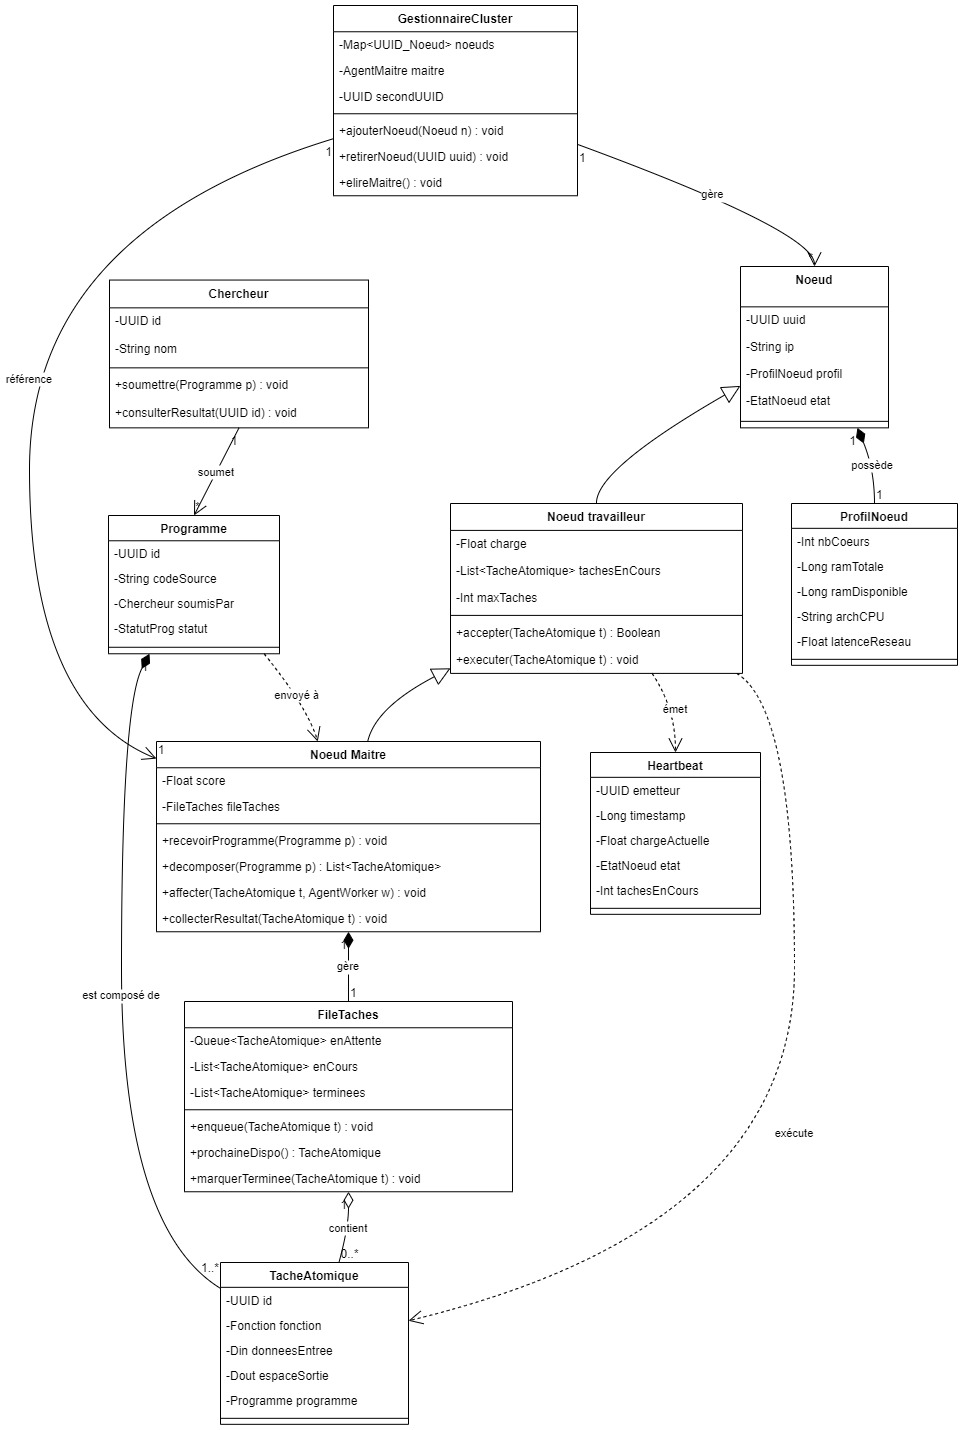
\includegraphics[width=1\textwidth]{images/parralax-classe technique.jpg}
            \caption{Diagramme de classe metiers }
            \label{fig:Diagramme de classes metiers}
        \end{figure}

    \subsubsection{diagramme de sequences Techniques}
            \begin{figure}[H]
            \centering
            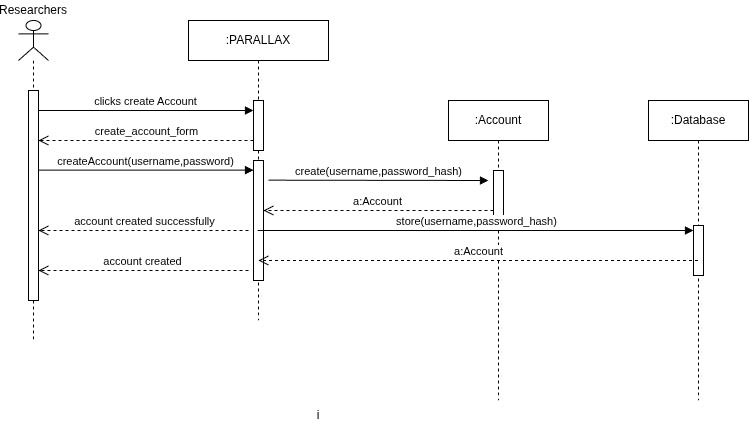
\includegraphics[width=1\textwidth]{images/parallax-AUTHENTIFCATION.jpg.jpeg}
            \caption{parallax-AUTHENTIFCATION}
            \label{fig:parallax-AUTHENTIFCATION}
        \end{figure}

        \begin{figure}[H]
            \centering
            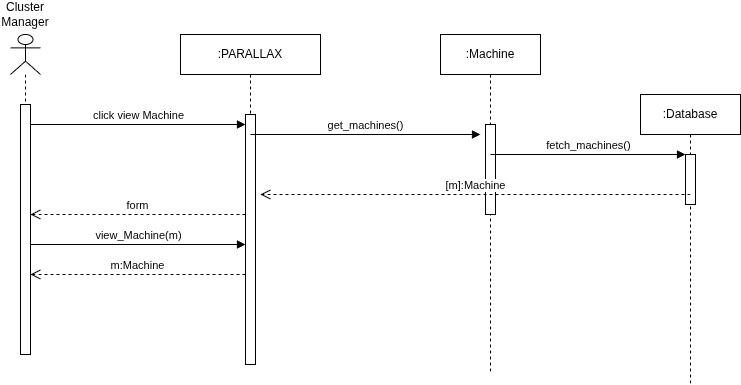
\includegraphics[width=1\textwidth]{images/parallax-consulter_machines (1).jpg.jpeg}
            \caption{consulter machines}
            \label{fig:consulter_machines}
        \end{figure}

        \begin{figure}[H]
            \centering
            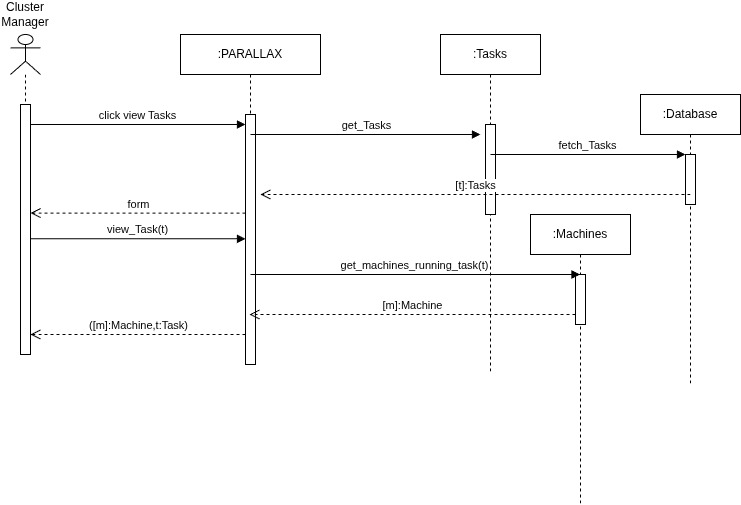
\includegraphics[width=1\textwidth]{images/parallax-consulter_taches (1).jpg.jpeg}
            \caption{consulter taches}
            \label{fig:consulter_taches}
        \end{figure}

        \begin{figure}[H]
            \centering
            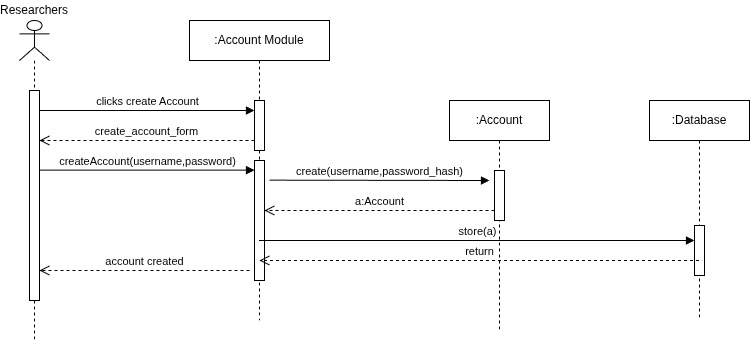
\includegraphics[width=1\textwidth]{images/parallax-CREATE_ACCOUNT.jpg.jpeg}
            \caption{CREATE ACCOUNT}
            \label{fig:CREATE_ACCOUNT}
        \end{figure}

        \begin{figure}[H]
            \centering
            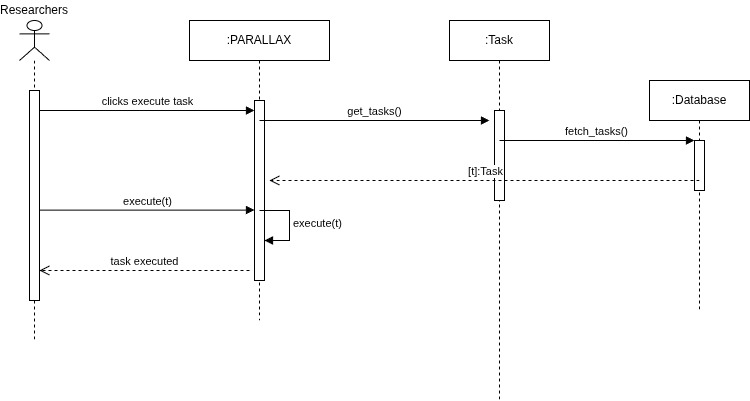
\includegraphics[width=1\textwidth]{images/parallax-ExecuteTask.jpg.jpeg}
            \caption{Execution de tache }
            \label{fig:Execution de tache}
        \end{figure}

        \begin{figure}[H]
            \centering
            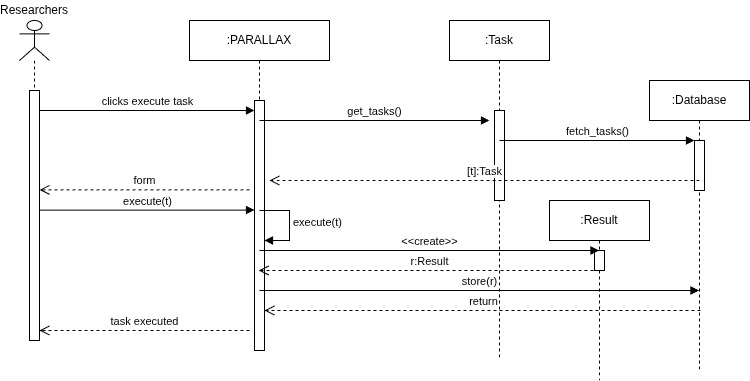
\includegraphics[width=1\textwidth]{images/parallax-ImportTask (2).jpg.jpeg}
            \caption{importer des taches }
            \label{fig:import des taches}
        \end{figure}

        \begin{figure}[H]
            \centering
            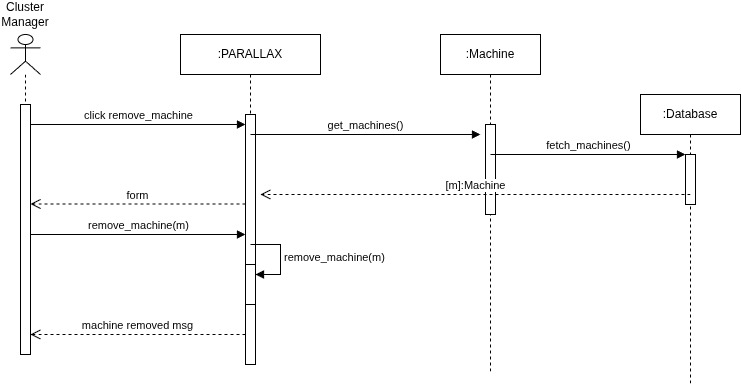
\includegraphics[width=1\textwidth]{images/parallax-Remove_Node.jpg.jpeg}
            \caption{enlever un noeud}
            \label{fig:enlever un noeud}
        \end{figure}

    \subsubsection{diagamme d'etats d'une tache}

        \begin{figure}[H]
            \centering
            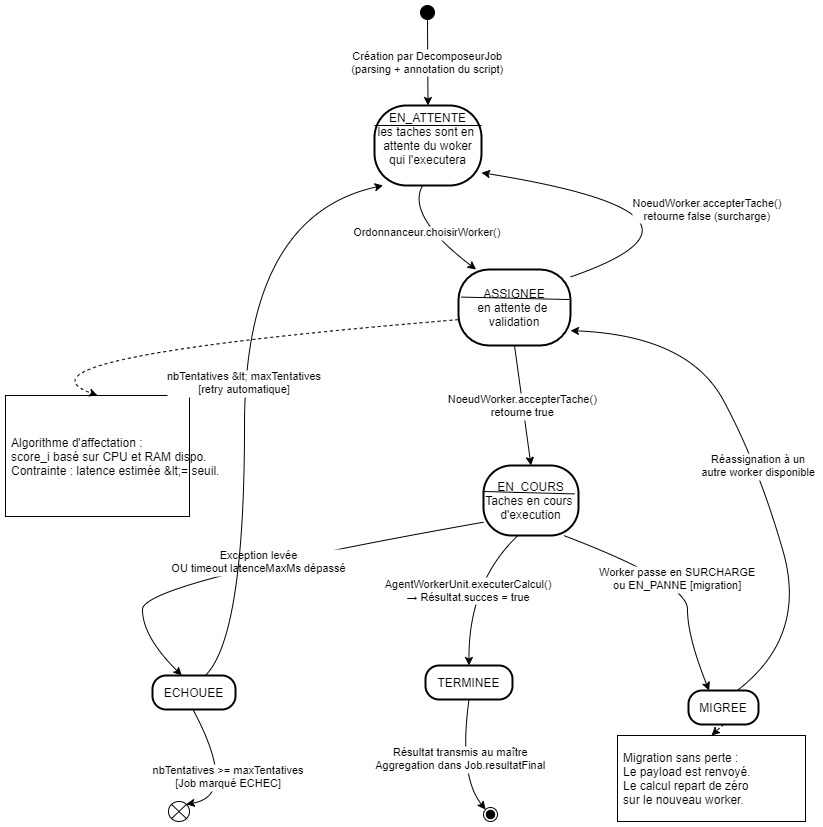
\includegraphics[width=1\textwidth]{images/parralax-etat d'une tache.jpg}
            \caption{Diagramme d'etat d'une tache }
            \label{fig:Diagramme d'etat d'une tache}
        \end{figure}
    
    \subsubsection{diagamme d'etats d'un noeud}

        \begin{figure}[H]
            \centering
            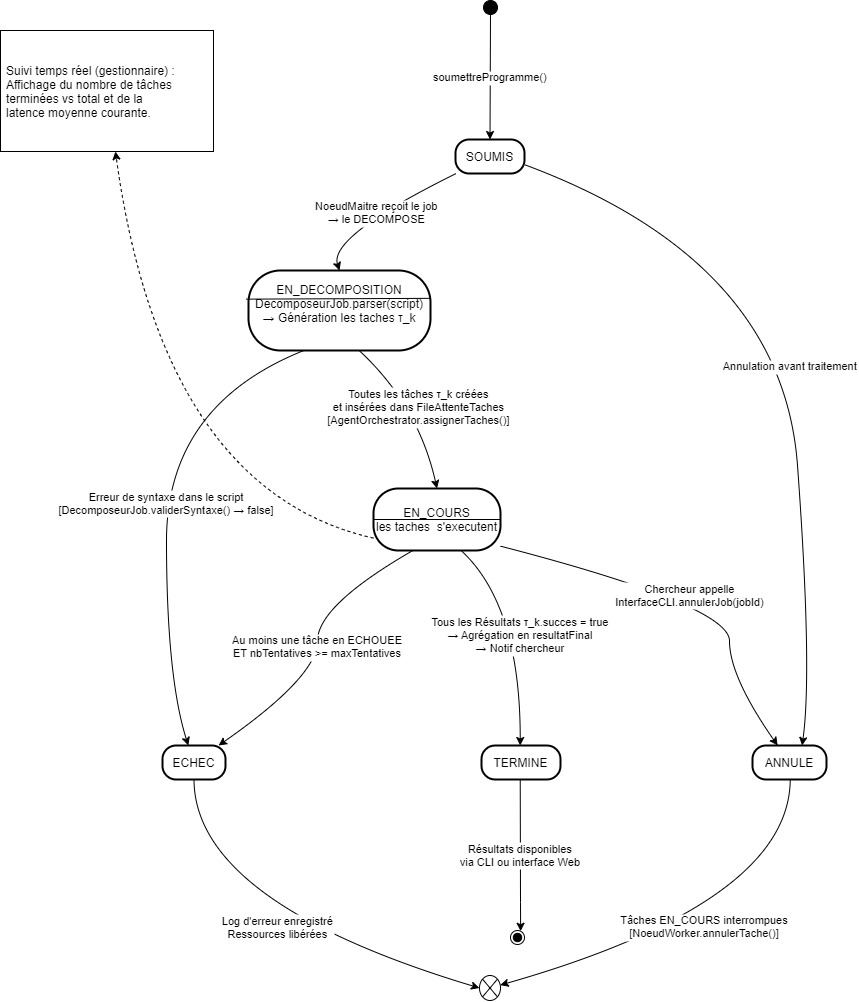
\includegraphics[width=1\textwidth]{images/parralax-etat d'un programme.jpg}
            \caption{Diagramme d'etat d'un programme}
            \label{fig:Diagramme d'etat d'un programme}
        \end{figure}
    
    \subsection{Diagramme d'etats}

    \begin{figure}[H]
        \centering
        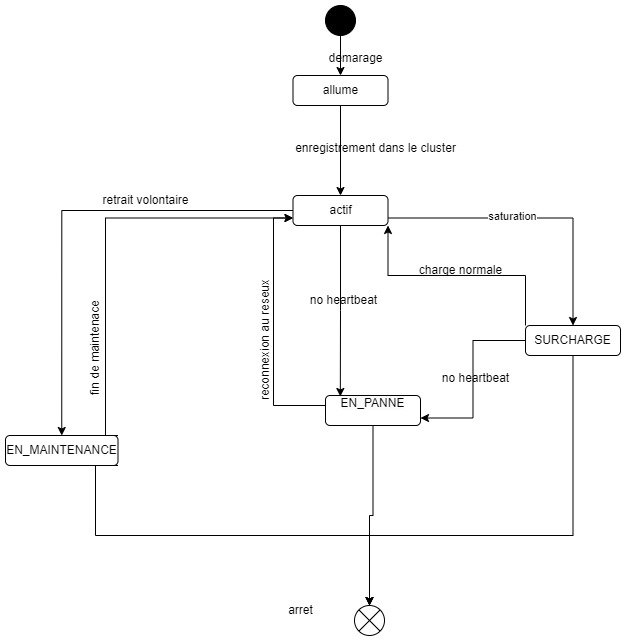
\includegraphics[width=1\textwidth]{images/parralax-etat d'un noeud.jpg}
        \caption{Diagramme d'etat d'un noeud}
        \label{fig:Diagramme d'etat d'un noeud}
    \end{figure}
    
    \subsection{ Diagramme des composants }

    \begin{figure}[H]
        \centering
        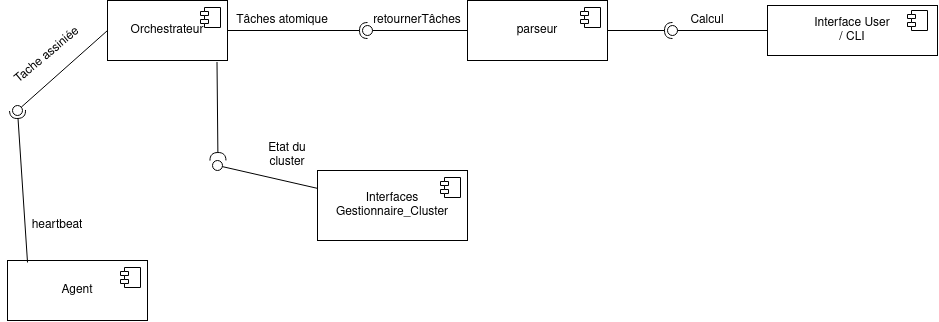
\includegraphics[width=1\textwidth]{images/Diagram des composants - parallax.drawio.png}
        \caption{Diagramme des composants - parallax}
        \label{fig:Diagramme des composants - parallax}
    \end{figure}

\chapter{Implémentation et Résultats}

\section{Outils et Technologies}
\section{Diagramme de Déploiement}
\section{Résultats}

\section*{Conclusion Générale}
\addcontentsline{toc}{chapter}{Conclusion  Générale}


\section*{Références}
\addcontentsline{toc}{chapter}{Références}

\begin{thebibliography}{99}

\bibitem{seti}
D. P. Anderson,
``SETI@home: An Experiment in Public-Resource Computing,''
\textit{Communications of the ACM}, vol. 45, no. 11, pp. 56--61, 2002.
doi: 10.1145/581571.581573.

\bibitem{snowball}
Amazon Web Services,
``AWS Snowball Documentation,''
2024. Available: \url{https://aws.amazon.com/snowball/}

\bibitem{spot}
P. Leitner and J. Cito,
``Patterns in the Chaos: A Study of Performance Variation and Predictability in Public IaaS Clouds,''
in \textit{Proc. ACM Int. Conf. on Cloud Engineering}, 2016, pp. 1--10.

\bibitem{htcondor}
D. Thain, T. Tannenbaum, and M. Livny,
``Distributed Computing in Practice: The Condor Experience,''
\textit{Concurrency and Computation: Practice and Experience}, vol. 17, no. 2--4, pp. 323--356, 2005.

\bibitem{tanenbaum_ds}
A. S. Tanenbaum and M. Van Steen,
\textit{Distributed Systems: Principles and Paradigms}, 2nd ed.
Prentice Hall, 2007.

\bibitem{wooldridge}
M. Wooldridge,
\textit{An Introduction to MultiAgent Systems}.
John Wiley \& Sons, 2009.

\bibitem{topcuoglu}
H. Topcuoglu, S. Hariri, and M.-Y. Wu,
``Performance-Effective and Low-Complexity Task Scheduling for Heterogeneous Computing,''
\textit{IEEE Trans. Parallel Distrib. Syst.}, vol. 13, no. 3, pp. 260--274, 2002.

\bibitem{kubernetes}
B. Burns, J. Beda, and K. Hightower,
\textit{Kubernetes: Up and Running}.
O'Reilly Media, 2019.

\bibitem{bully}
H. Garcia-Molina,
``Elections in a Distributed Computing System,''
\textit{IEEE Trans. Computers}, vol. C-31, no. 1, pp. 48--59, 1982.

\end{thebibliography}
\section*{Annexes}

\end{document}

\end{document}
